\documentclass[10pt]{article}

\usepackage[latin1]{inputenc}
\usepackage{amsmath, amssymb, amsfonts, amsthm}
\usepackage{upgreek}
\usepackage{amsthm}
\usepackage{fullpage}
\usepackage{graphicx}
\usepackage{cancel}
\usepackage{subfigure}
\usepackage{mathrsfs}
%\usepackage{outlines}
\usepackage[font={sf,it}, labelfont={sf,bf}, labelsep=space, belowskip=5pt]{caption}
\usepackage{hyperref}
\usepackage{minted}

\usepackage{fancyhdr}
\usepackage[title]{appendix}
\usepackage{titling}

\DeclareMathOperator{\sgn}{sgn}

\pagestyle{fancy}
\headheight 24pt
\headsep    12pt
\lhead{Exploration of Homogenization}
\fancyfoot[C]{} % hide the default page number at the bottom
\lfoot{}
\rfoot{\thepage}
\renewcommand{\headrulewidth}{0.4pt}
\renewcommand\footrulewidth{0.4pt}
\providecommand{\abs}[1]{\lvert#1\rvert}
\providecommand{\norm}[1]{\lVert#1\rVert}
\providecommand{\dx}{\, \mathrm{d}x}
% \providecommand{\vint}[2]{\int_{#1} \! #2 \, \mathrm{d}x}
% \providecommand{\sint}[2]{\int_{\partial #1} \! #2 \, \mathrm{d}A}
\renewcommand{\div}{\nabla \cdot}
\providecommand{\shape}{\Omega(p)}
\providecommand{\boundary}{\partial \shape}
\providecommand{\vint}[1]{\int_{\shape} \! #1 \, \mathrm{d}x}
\providecommand{\sint}[1]{\int_{\boundary} \! #1 \, \mathrm{d}A}
\providecommand{\pder}[2]{\frac{\partial #1}{\partial #2}}
\providecommand{\tder}[2]{\frac{\mathrm{d} #1}{\mathrm{d} #2}}
\providecommand{\evalat}[2]{\left.#1\right|_{#2}}
\newcommand{\defeq}{\vcentcolon=}
\newtheorem{lemma}{Lemma}

\makeatletter
\usepackage{mathtools}
\newcases{mycases}{\quad}{%
  \hfil$\m@th\displaystyle{##}$}{$\m@th\displaystyle{##}$\hfil}{\lbrace}{.}
\makeatother

\title{Homogenization of Sequential Laminates}
\author{Julian Panetta and Qingnan Zhou}

% BEGIN DOCUMENT
\begin{document}

\setlength{\droptitle}{-50pt}
\maketitle

We attempt to visualize the space of possible homogenized elasticity tensors of
sequential laminates of two isotropic base materials in $2D$. All definitions
come from \cite{allaire2002shape}. Let $A$ and $B$ be the materials' elasticity
tensors, specified by Lam\'e parameters $\mu_A,\ \lambda_A,\ \mu_B,\ $ and
$\lambda_B$. We then sequentially perform $p$ steps of lamination of $B$ with
layers of $A$ in directions $e_i \in \mathbb{R}^2$ and with densities $\theta_i \in
(0, 1)$ ($\theta_i = 0$ and $\theta_i = 1$ mean a homogenous material and aren't
considered).

\section{Formula Derivations}
The resulting homogenized elasticity tensor, $A^*_p$ is given by:
\begin{align}
\label{eqn:Astar}
\left(\prod_{i=1}^p (1 - \theta_i) \right)\left(A^*_p - A\right)^{-1} =
\left(B - A\right)^{-1} + \sum_{i = 1}^p
\left( \theta_i \prod_{j = 1}^{i - 1} (1 - \theta_j)\right) f_A(e_i)
\end{align}

Where $f_A$ is defined by its action on a symmetric stress tensor $\sigma$:
\begin{align}
f_A(e) \sigma \defeq \frac{1}{2\mu_A} \left(\sigma e e^T + e e^T \sigma^T \right)
    + \left(\frac{1}{2 \mu_A  + \lambda_A} - \frac{1}{\mu_A}\right)\left(
    (e^T \sigma e) e e^T \right)
\label{eqn:fAdef}
\end{align}
or, in index notation, with $F \defeq f_A(e)$:
$$
F_{ijkl} \sigma_{kl} = \frac{1}{2\mu_A} \left(\sigma_{im} e_m e_j + \sigma_{jm} e_m e_i \right)
    + \left(\frac{1}{2 \mu_A  + \lambda_A} - \frac{1}{\mu_A}\right)\left(
    \sigma_{mn} e_m e_n e_i e_j \right).
$$
By inspection (easily verified), we see that one possible such tensor is:
$$
\overline{F}_{ijkl} = \frac{1}{2 \mu_A} (\delta_{ki} e_l e_j + \delta_{kj} e_l e_i) +
\left(\frac{1}{2 \mu_A + \lambda_A} - \frac{1}{\mu_A}\right)(e_i e_j e_k e_l).
$$
However, this is not the only possible tensor because definition (\ref{eqn:fAdef}) is
incomplete. Since $f_A(e)$ is only defined by its
action on symmetric matrices, the exact $F_{ijkl}$ is not completely specified;
really only the sum $F_{ijkl} + F_{ijlk}$ is pinned down. This is because each
of those terms gets the same weight in the contraction: $2 F_{ijkl} \sigma_{kl} =
F_{ijkl} (\sigma_{kl} + \sigma_{lk}) =
F_{ijkl} \sigma_{kl} + F_{ijkl}\sigma_{lk} =
F_{ijkl} \sigma_{kl} + F_{ijlk}\sigma_{kl} =  
(F_{ijkl} + F_{ijlk})\sigma_{kl}$.
Thus we can choose the single tensor that is symmetric in $k$ and $l$: $F_{ijkl}
= \frac{1}{2}(\overline{F}_{ijkl} + \overline{F}_{ijlk})$. Together with the
fact that $f_A$ always maps to symmetric matrices (transposing the
RHS of (\ref{eqn:fAdef}) gives the same expression), this means our chosen
$F_{ijkl}$ has the same minor symmetries as an elasticity tensor. This is more
than just a convenience: since $A^*_p$, $A$, and $B$ are all symmetric in their
minors, (\ref{eqn:Astar}) seems to require $f_A$ have the same symmetry. The
full expression for $f_A$ in index notation is:
$$
F_{ijkl} = 
\frac{1}{4 \mu_A} (\delta_{ki} e_l e_j + \delta_{kj} e_l e_i + \delta_{li} e_k e_j + \delta_{lj} e_k e_i) +
\left(\frac{1}{2 \mu_A + \lambda_A} - \frac{1}{\mu_A}\right)(e_i e_j e_k e_l).
$$

Since $F_{ijkl}$ is a linear map from symmetric matrices to symmetric matrices,
we can express it using a variant of Voigt notation where strain is represented
as the vector $(\epsilon_{11}, \epsilon_{22}, \epsilon_{12})^T$ (i.e.
non-engineering strain). This allows us to do the
same for $A$, $B$, and $A^*_p$ in (\ref{eqn:Astar}) so that the tensor inverses
simply become $3\times3$ matrix inverses. The matrix version of $f_A(e)$ is:

$$
\mathcal{F} = \begin{pmatrix} F_{1111} & F_{1122} & F_{1112} \\ 
                              F_{2211} & F_{2222} & F_{2212} \\
                              F_{1211} & F_{1222} & F_{1212} \end{pmatrix}
% From Mathematica:
% FirstMat_{1111}= 4 e_1^2
% FirstMat_{1122}= 0
% FirstMat_{1112}= 2 e_1 e_2
% FirstMat_{2211}= 0
% FirstMat_{2222}= 4 e_2^2
% FirstMat_{2212}= 2 e_1 e_2
% FirstMat_{1211}= 2 e_1 e_2
% FirstMat_{1222}= 2 e_1 e_2
% FirstMat_{1212}= e_1^2+e_2^2
= \frac{1}{4 \mu_A}
 \begin{pmatrix}  4 e_1^2   &  0         &  2 e_1 e_2   \\
                  0         &  4 e_2^2   &  2 e_1 e_2   \\
                  2 e_1 e_2 &  2 e_1 e_2 &  e_1^2+e_2^2 \end{pmatrix}
+ \left(\frac{1}{2 \mu_A + \lambda_A} - \frac{1}{\mu_A}\right)
  \begin{pmatrix} e_1^4 & e_1^2 e_2^2 & e_1^3 e_2 \\ 
                              e_1^2 e_2^2 & e_2^4 & e_1 e_2^3 \\
                              e_1^3 e_2 & e_1 e_2^3 & e_1^2 e_2^2 \end{pmatrix}
$$
It is finally apparent that $fA(e)$ has the same major symmetry as an elasticity
tensor: $\mathcal{F} = \mathcal{F}^T$. This is important since it ensures
the required major symmetry in homogenized elasticity tensor $A^*_p$ by
(\ref{eqn:Astar}).

Isotropic elasticity tensors implement the linear Hooke's law $\sigma = \lambda
tr(\epsilon) I + 2 \mu \epsilon$. Thus, in our notation, $A$ and $B$ are:
$$
    A = \begin{pmatrix}
        \lambda_A + 2 \mu_A & \lambda_A         & 0 \\
        \lambda_A         & \lambda_A + 2 \mu_A & 0 \\
        0               & 0               & 2 \mu_A
        \end{pmatrix},\quad
    B = \begin{pmatrix}
        \lambda_B + 2 \mu_B & \lambda_B         & 0 \\
        \lambda_B         & \lambda_B + 2 \mu_B & 0 \\
        0               & 0               & 2 \mu_B
        \end{pmatrix}.
$$

\section{Numerical Exploration}
Here we numerically explore the homogenized elasticity tensors $A^*_p$ by
trying $N_\theta$ evenly spaced values for $\theta_i$ and $e_i = (\cos(\alpha_i),\
\sin(\alpha_i))^T$ for $N_e$ evenly spaced angles $\alpha \in [0, \pi)$; we only
need to cover half the unit circle because $-e_i$ gives the same
laminate as $e_i$. We also try $p = 1, 2, 3 \dots$ lamination steps. When $p$
steps are employed, the total number of parameter combinations is $(N_\theta *
N_e)^p$. For each combination we need to evaluate the following expression:
\begin{align}
\label{eqn:AstarSolve}
A^*_p = A + \left( \prod_{i=1}^p (1 - \theta_i) \right)
\left[\left(B - A\right)^{-1} + \sum_{i = 1}^p
\left( \theta_i \prod_{j = 1}^{i - 1} (1 - \theta_j)\right) f_A(e_i)\right]^{-1}
\end{align}
$(B - A)^{-1}$ can be precomputed, so each iteration involves a single $3 \times
3$ matrix inverse after accumulating the linear combination of $f_A(e_i)$.

We also need to search over parameters for $\lambda_A$, $\mu_A$, $\lambda_B$,
and $\mu_B$, satisfying $\mu_A \le \mu_B$ and $\kappa_A \le \kappa_B$, where
$$
 \kappa = \lambda + 2\frac{\mu}{N} = \lambda + \mu
$$
This search is more easily analyzed by changing parameters to Young's modulus,
$E$, and Poisson ratio, $\nu$:
$$
\mu = \frac{E}{2(1 + \nu)}, \quad
\kappa = \frac{E}{2(1 - \nu)}, \quad
\lambda = \kappa - \mu = \frac{E(1 + \nu) - E(1 - \nu)}{2(1 + \nu)(1 - \nu)}
= \frac{E \nu}{(1 + \nu)(1 - \nu)}.
% \lambda = \frac{E \nu}{(1 + \nu)(1 - 2\nu)}.
$$
where the $2D$ conversion formulas were taken from \cite{jasiuk}.
The first thing we notice is that $\lambda, \mu \propto E$. This means $A$ and
$B$ are also $\propto$ $E_A$ and $E_B$ respectively, and $f_A(e) \propto
\frac{1}{E_A}$ by (\ref{eqn:fAdef}).
Finally, from (\ref{eqn:AstarSolve}), if we choose scaled $E_A' = \alpha E_A$
and $E_B' = \alpha E_B$, then $A_p^{*\prime} = \alpha A_p^*$. So, without loss of
generality we can take $E_A = 1$; all homogenizations can be computed
by scaling the elasticity tensor computed for $E_A' = 1$ and $E_B' =
\frac{E_B}{E_A}$ by $E_A$. Moreover, we must have $E_B > E_A$.
\begin{proof}
    Choose $E_A > E_B$. Then to satisfy $\mu_A \le \mu_B$, the conversion
    formulas tell us we must have $\nu_A > \nu_B$. But, to satisfy $\kappa_A \le
    \kappa_B$, we must have $\nu_A < \nu_B$. Hence, there is no choice for
    $\nu_A$ and $\nu_B$ that achieves a valid material pair when $E_A > E_B$.
    Now, when $E_A = E_B$, in order to get two distinct materials, obviously
    $\nu_A \ne \nu_B$. But then either $\kappa_A > \kappa_B$ or $\mu_A > \mu_B$
    and no valid material pair is possible.
\end{proof}
This means, without loss of generality we can look in the range $(1, \infty]$
for $E_B$. We choose to restrict our search to the range $(1, 10]$, asserting
that material $B$ is at most $10\times$ stronger than $A$. For $\nu_A$ and
$\nu_B$, we search the range $(-1, .5)$ and throw out any invalid resulting
material pairs. Considering $N_E$ evenly spaced $E_B$s and $N_\nu$ evenly spaced
$\nu_A$s and $\nu_B$s, this means homogenizing at most $N_E N_\nu^2$ material
pairs:
\inputminted[linenos,fontsize=\footnotesize]{matlab}{materialScan.m}

% The code to perform the search is:
% \inputminted[linenos,fontsize=\footnotesize]{matlab}{sequentialLaminates.m}

\section{Visualization}
The symmetric homogenized tensor is a point in $\mathbb{R}^6$. Unfortunately,
this is very hard to visualize. To simplify things, we consider only tensors
approximating isotropic tensors since those are a 2D subspace that is easily
parameterized and visualized. Thus we can plot on a $(\lambda, \mu)$ plane. We
color points based on $p$ value.

\section{Results}
For each homogenized material tensor $A^*_p$, we find the best fitting isotropic
material tensor, $A_{\textrm{fit}}$, in the least square sense.  
The residual error, $E_{\textrm{fit}}$, is define as
$$
E_{\textrm{fit}} = \frac{\|A^*_p -
A_{\textrm{fit}}\|_{\textrm{fro}}}{\|A_{\textrm{fit}}\|_{\textrm{fro}}}
$$
The corresponding isotropic material properties can be extracted from
$A_{\textrm{fit}}$.

\begin{figure}
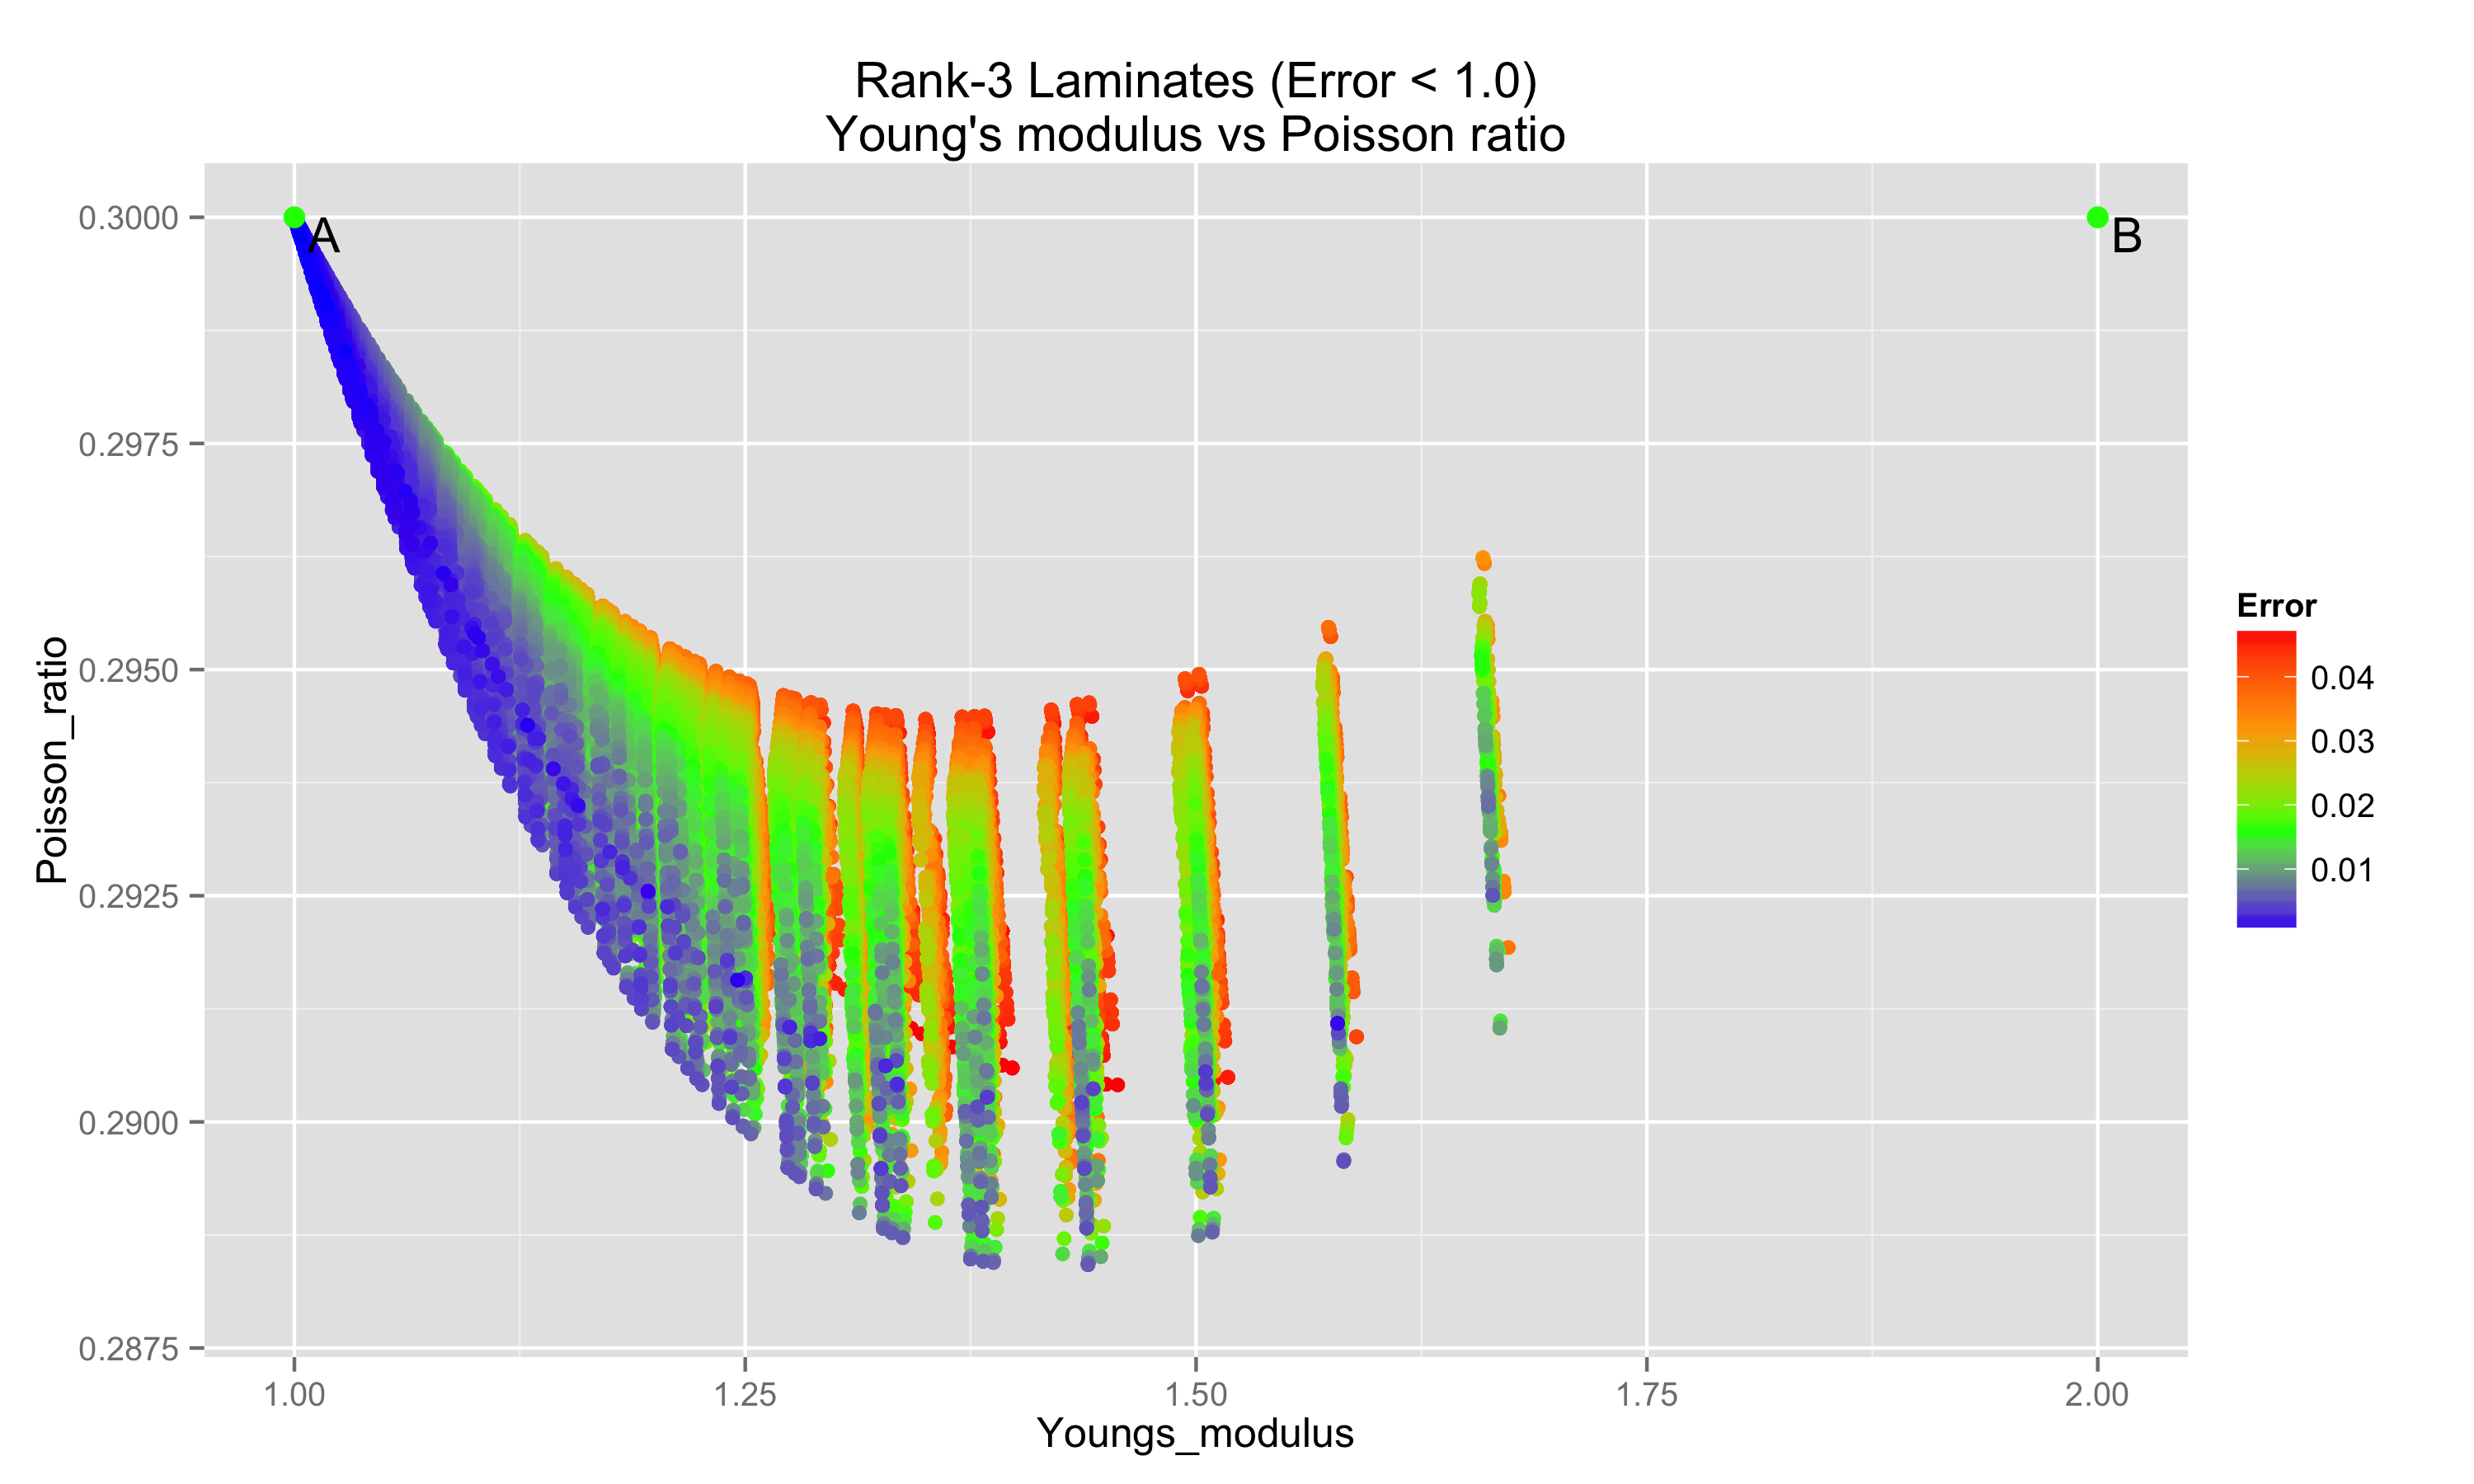
\includegraphics[width=0.49\textwidth]{{images/p3_e1.0_young_poisson_error}.png}
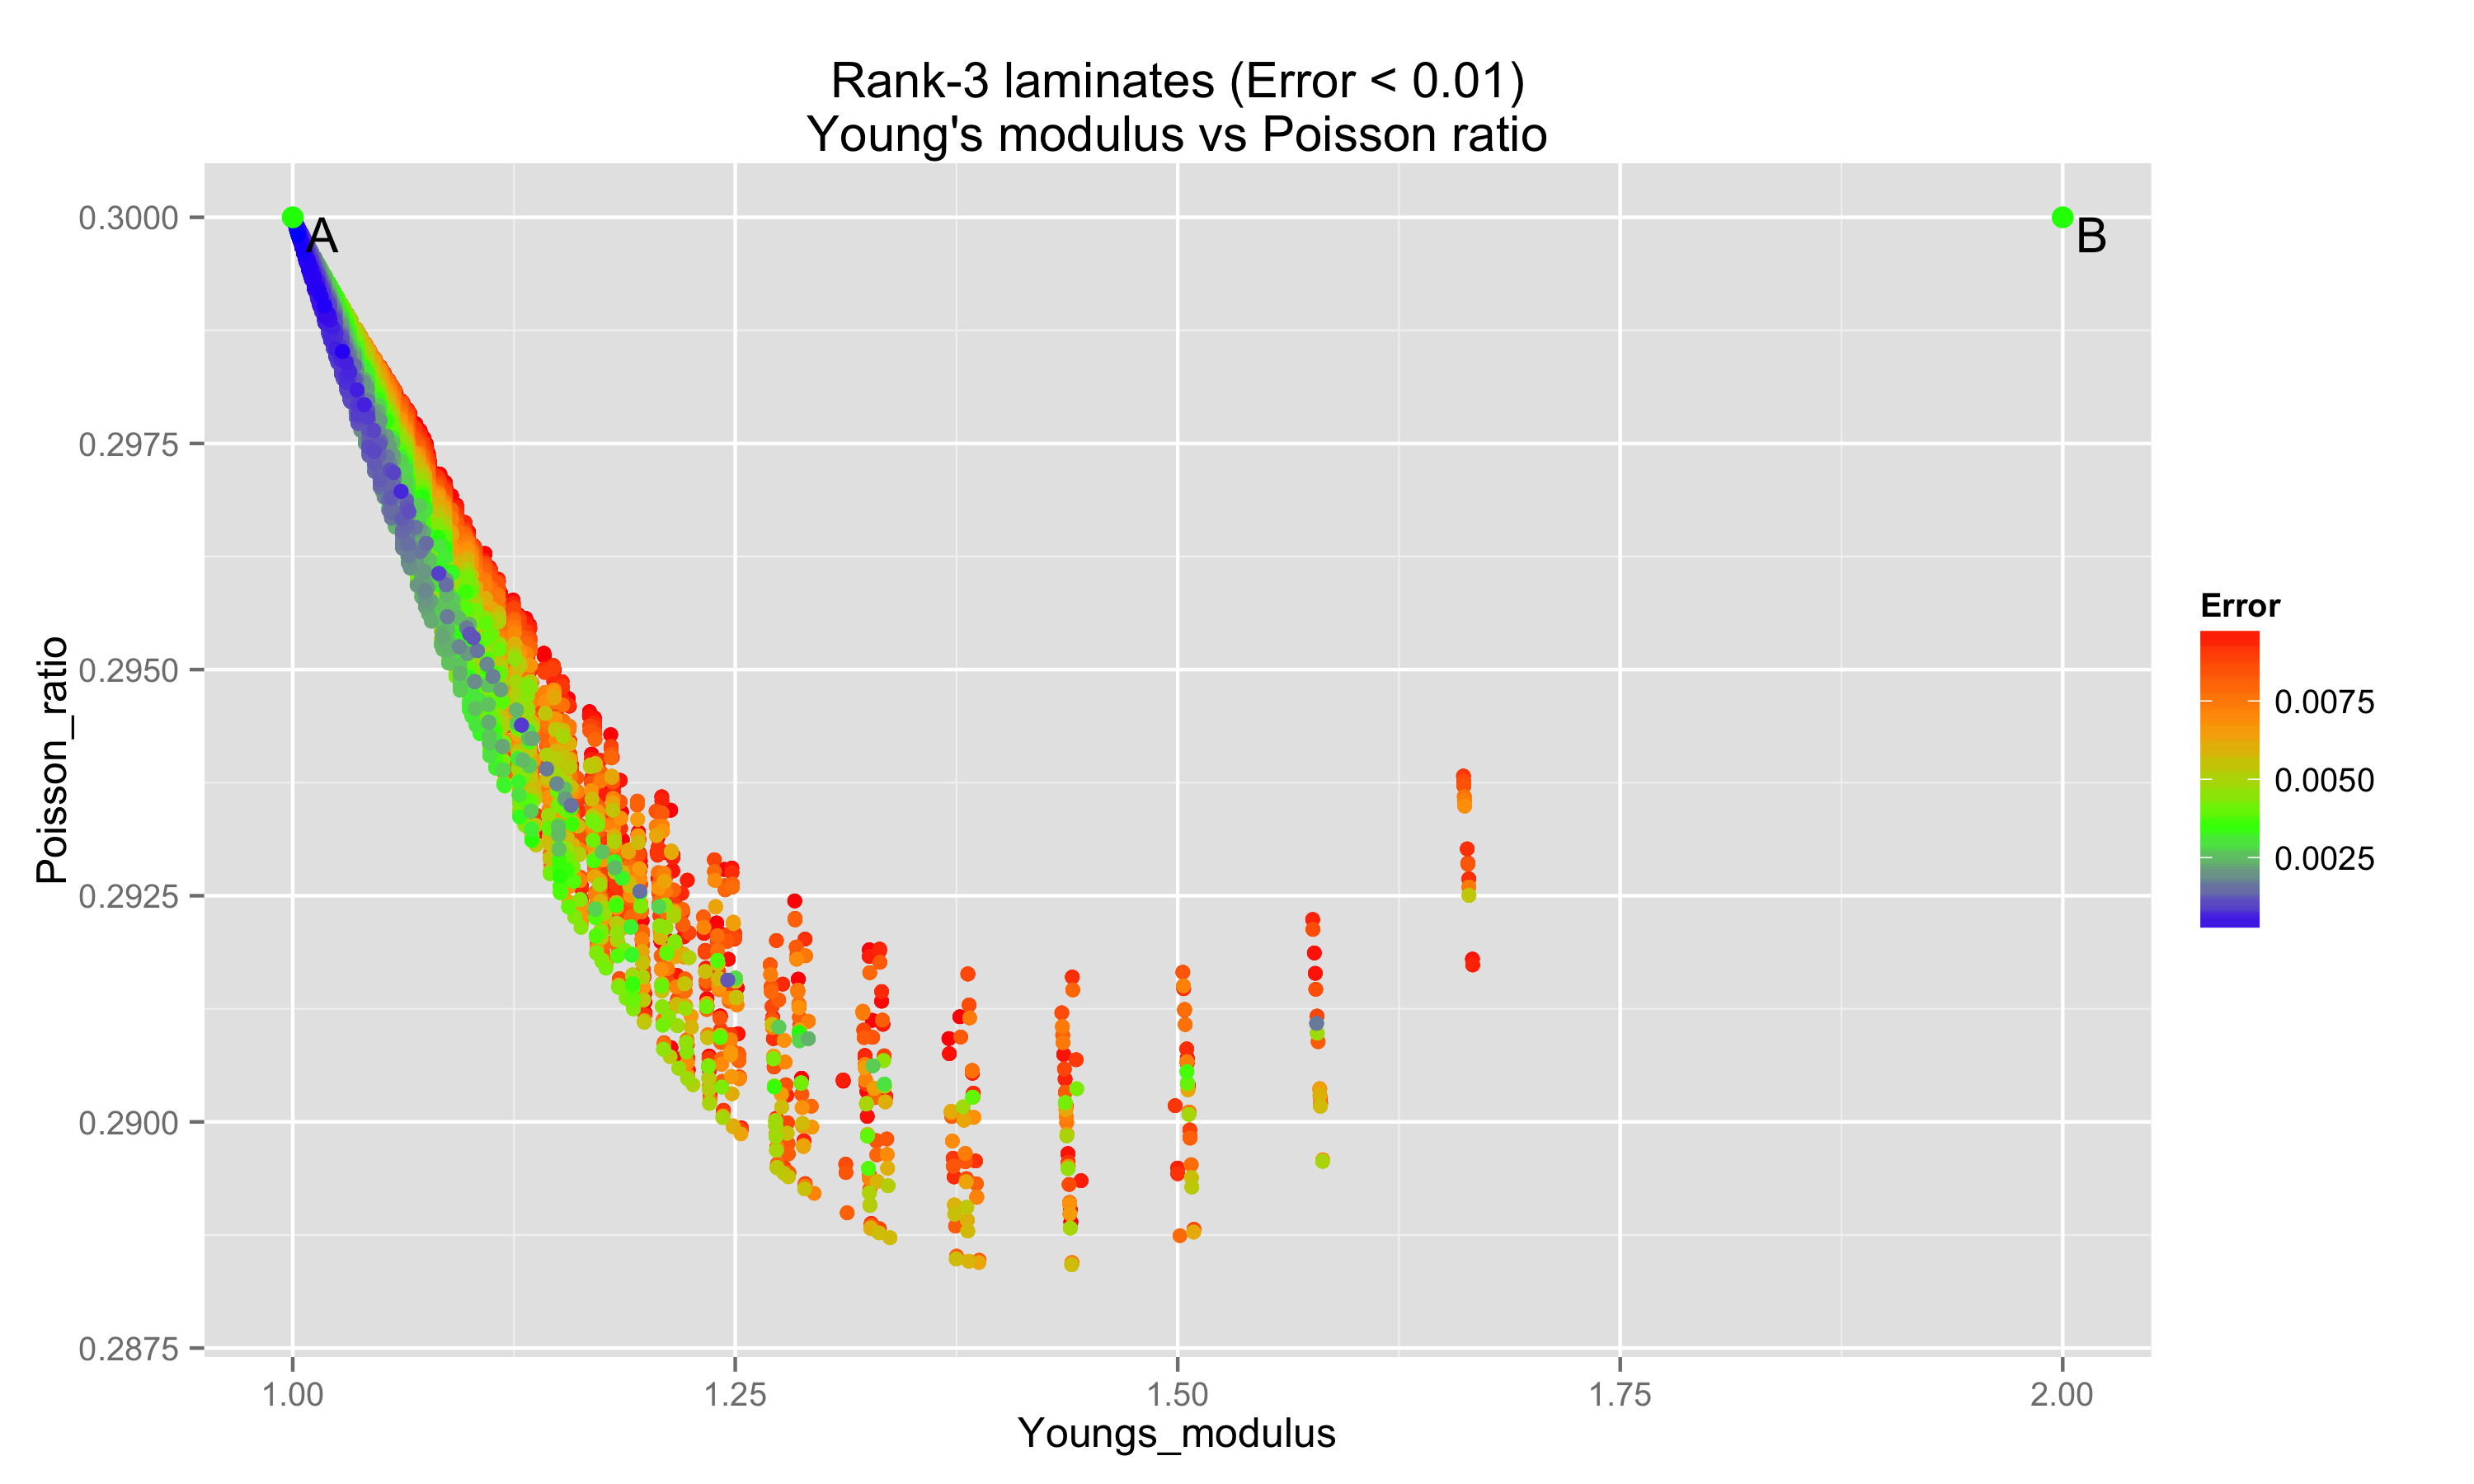
\includegraphics[width=0.49\textwidth]{{images/p3_e0.01_young_poisson_error}.png}
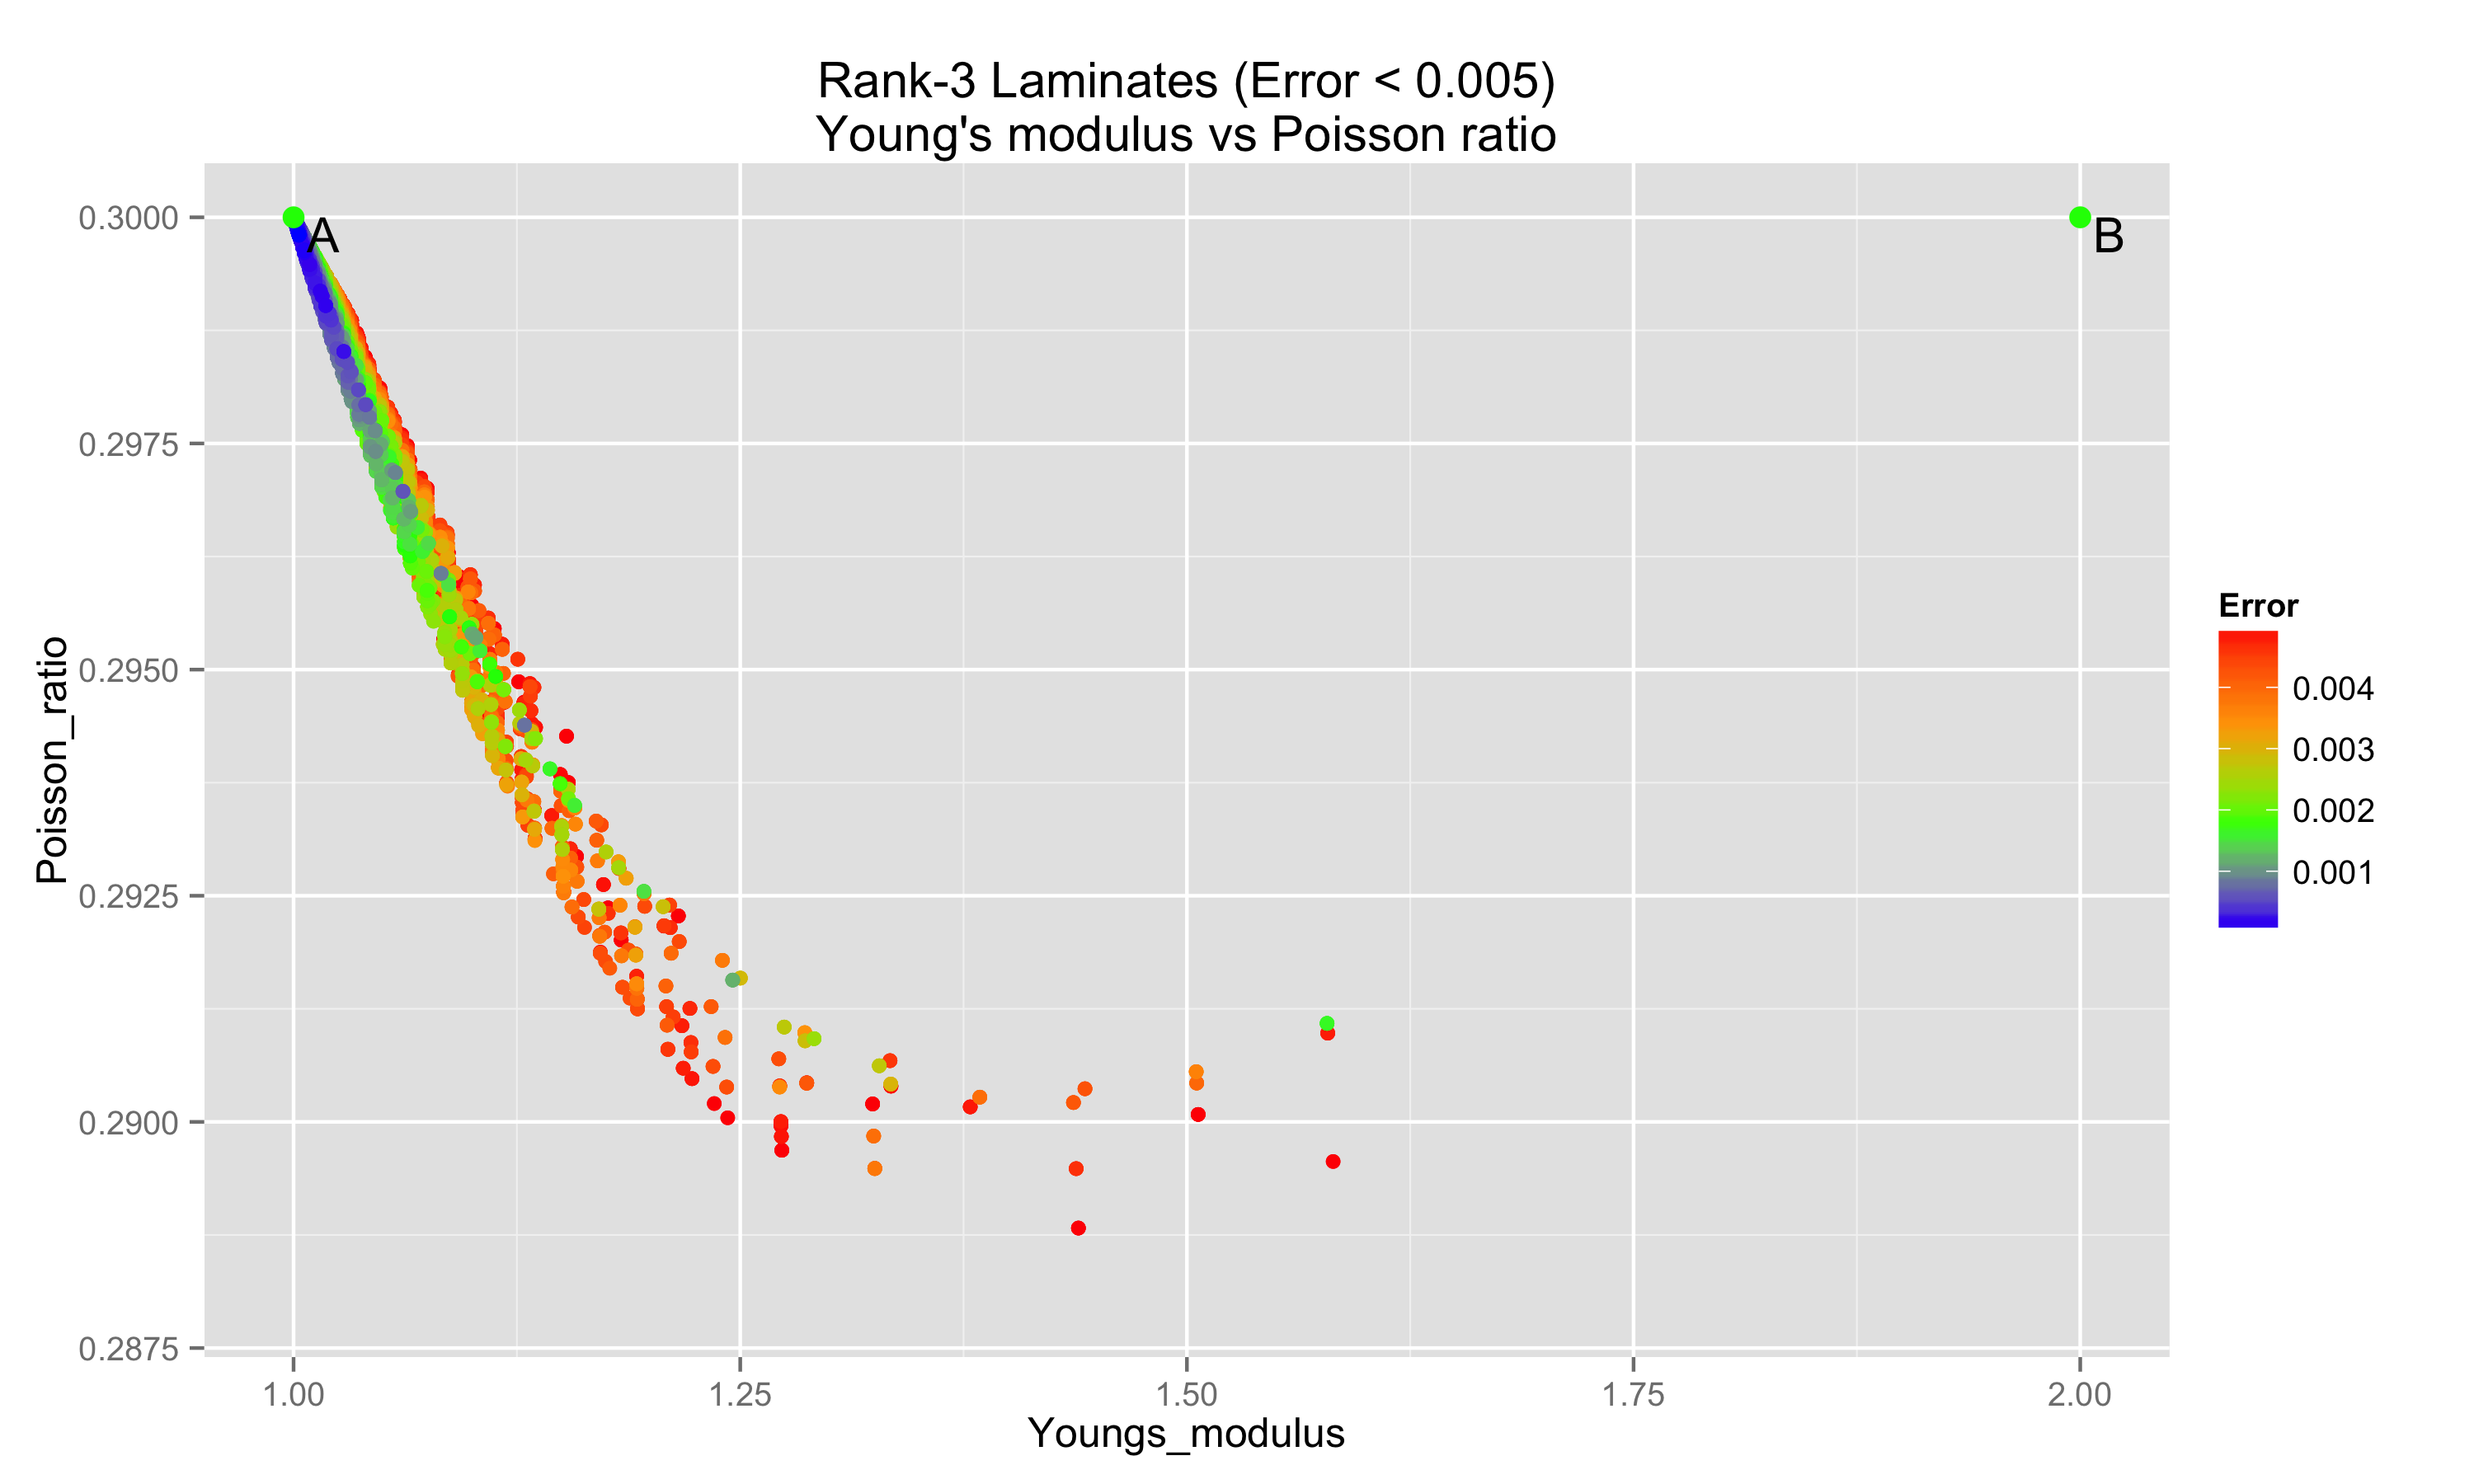
\includegraphics[width=0.49\textwidth]{{images/p3_e0.005_young_poisson_error}.png}
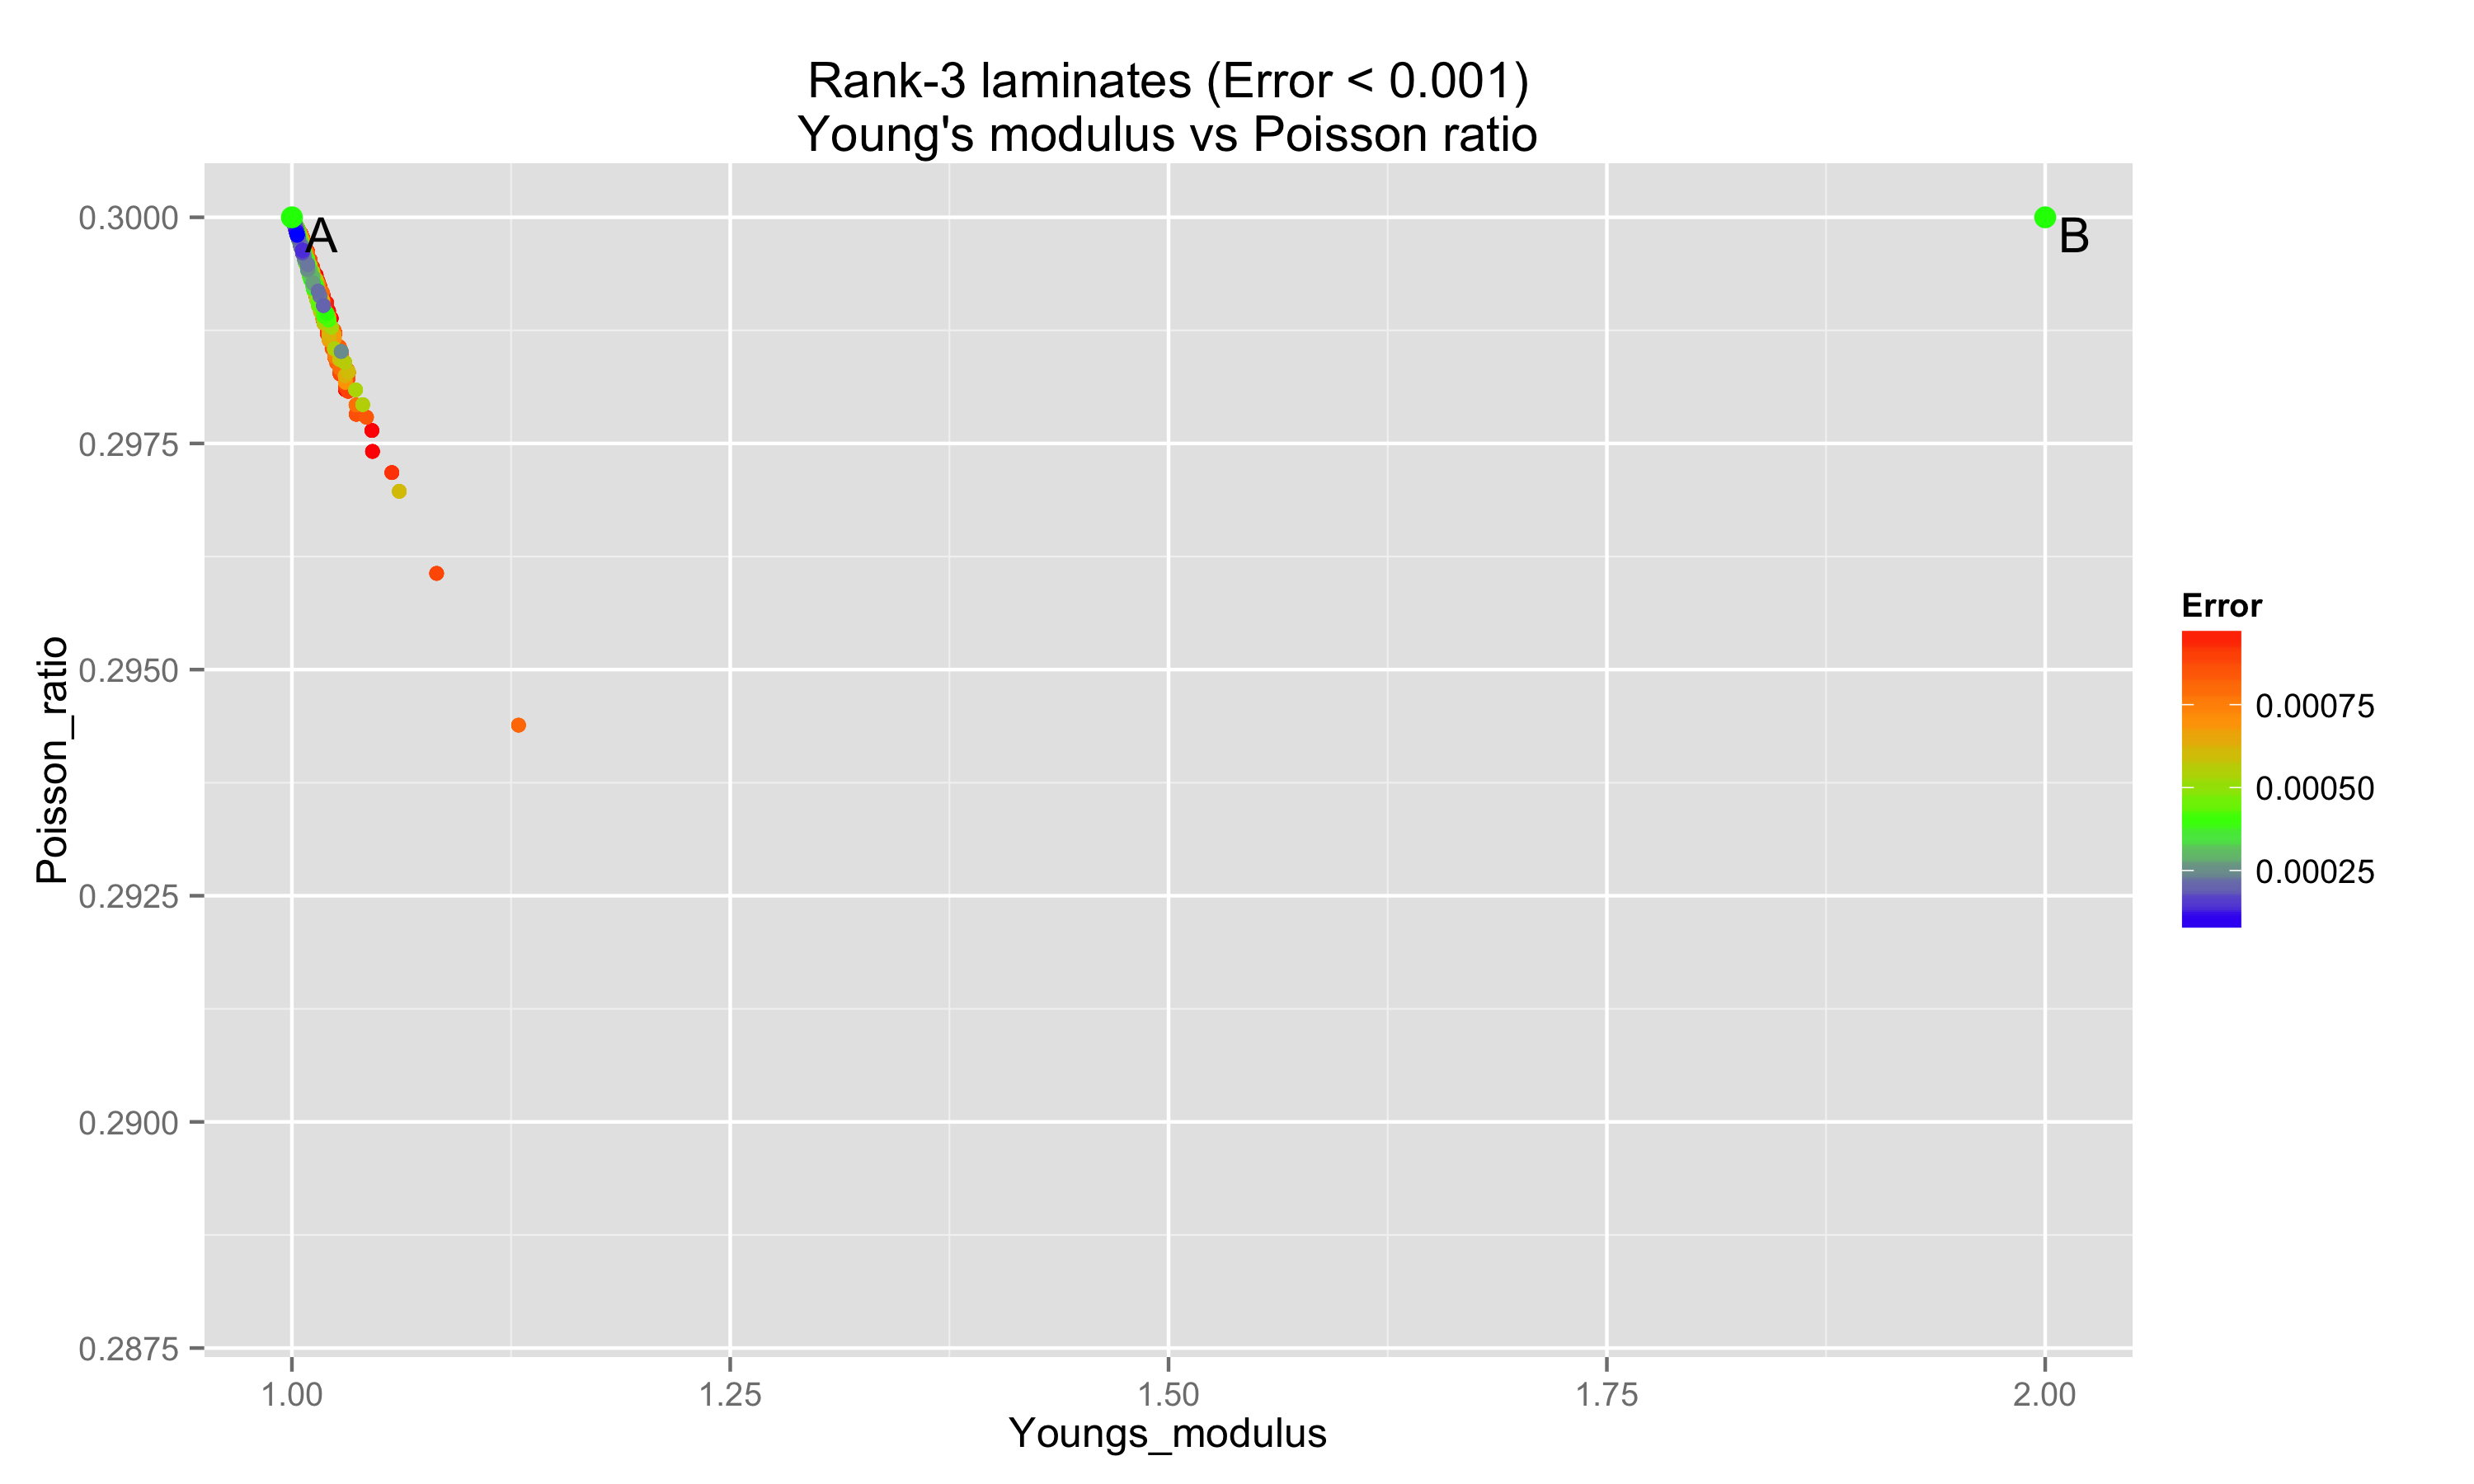
\includegraphics[width=0.49\textwidth]{{images/p3_e0.001_young_poisson_error}.png}
\caption{ Homogenized material tensors for rank-3 laminates visualized in Young's
modulus vs Poisso ratio space.  Top left: all tensors are plotted.  Top right:
$E_{\textrm{fit}} < 0.01$.  Bottom left: $E_{\textrm{fit}} < 0.005$.  Bottom
right: $E_{\textrm{fit}} < 0.001$. }
\label{fig:rank3_error}
\end{figure}

As shown in Figure \ref{fig:rank3_error} (top left), all sampled rank-3 material
tensors are plotted where $E_{\textrm{fit}}$ maps to color.  They occupies a
crecent shape region with one end correponding to $A$, and the other end can be
extrapolated to $B$.  Unsupprisingly most samples are concentrated near the
the weaker base material $A$.  As we filter out samples with large errors,
Figure \ref{fig:rank3_error} top right and bottom, we see that the lower arc of
the crecent has the lowest fitting error.

\begin{figure}
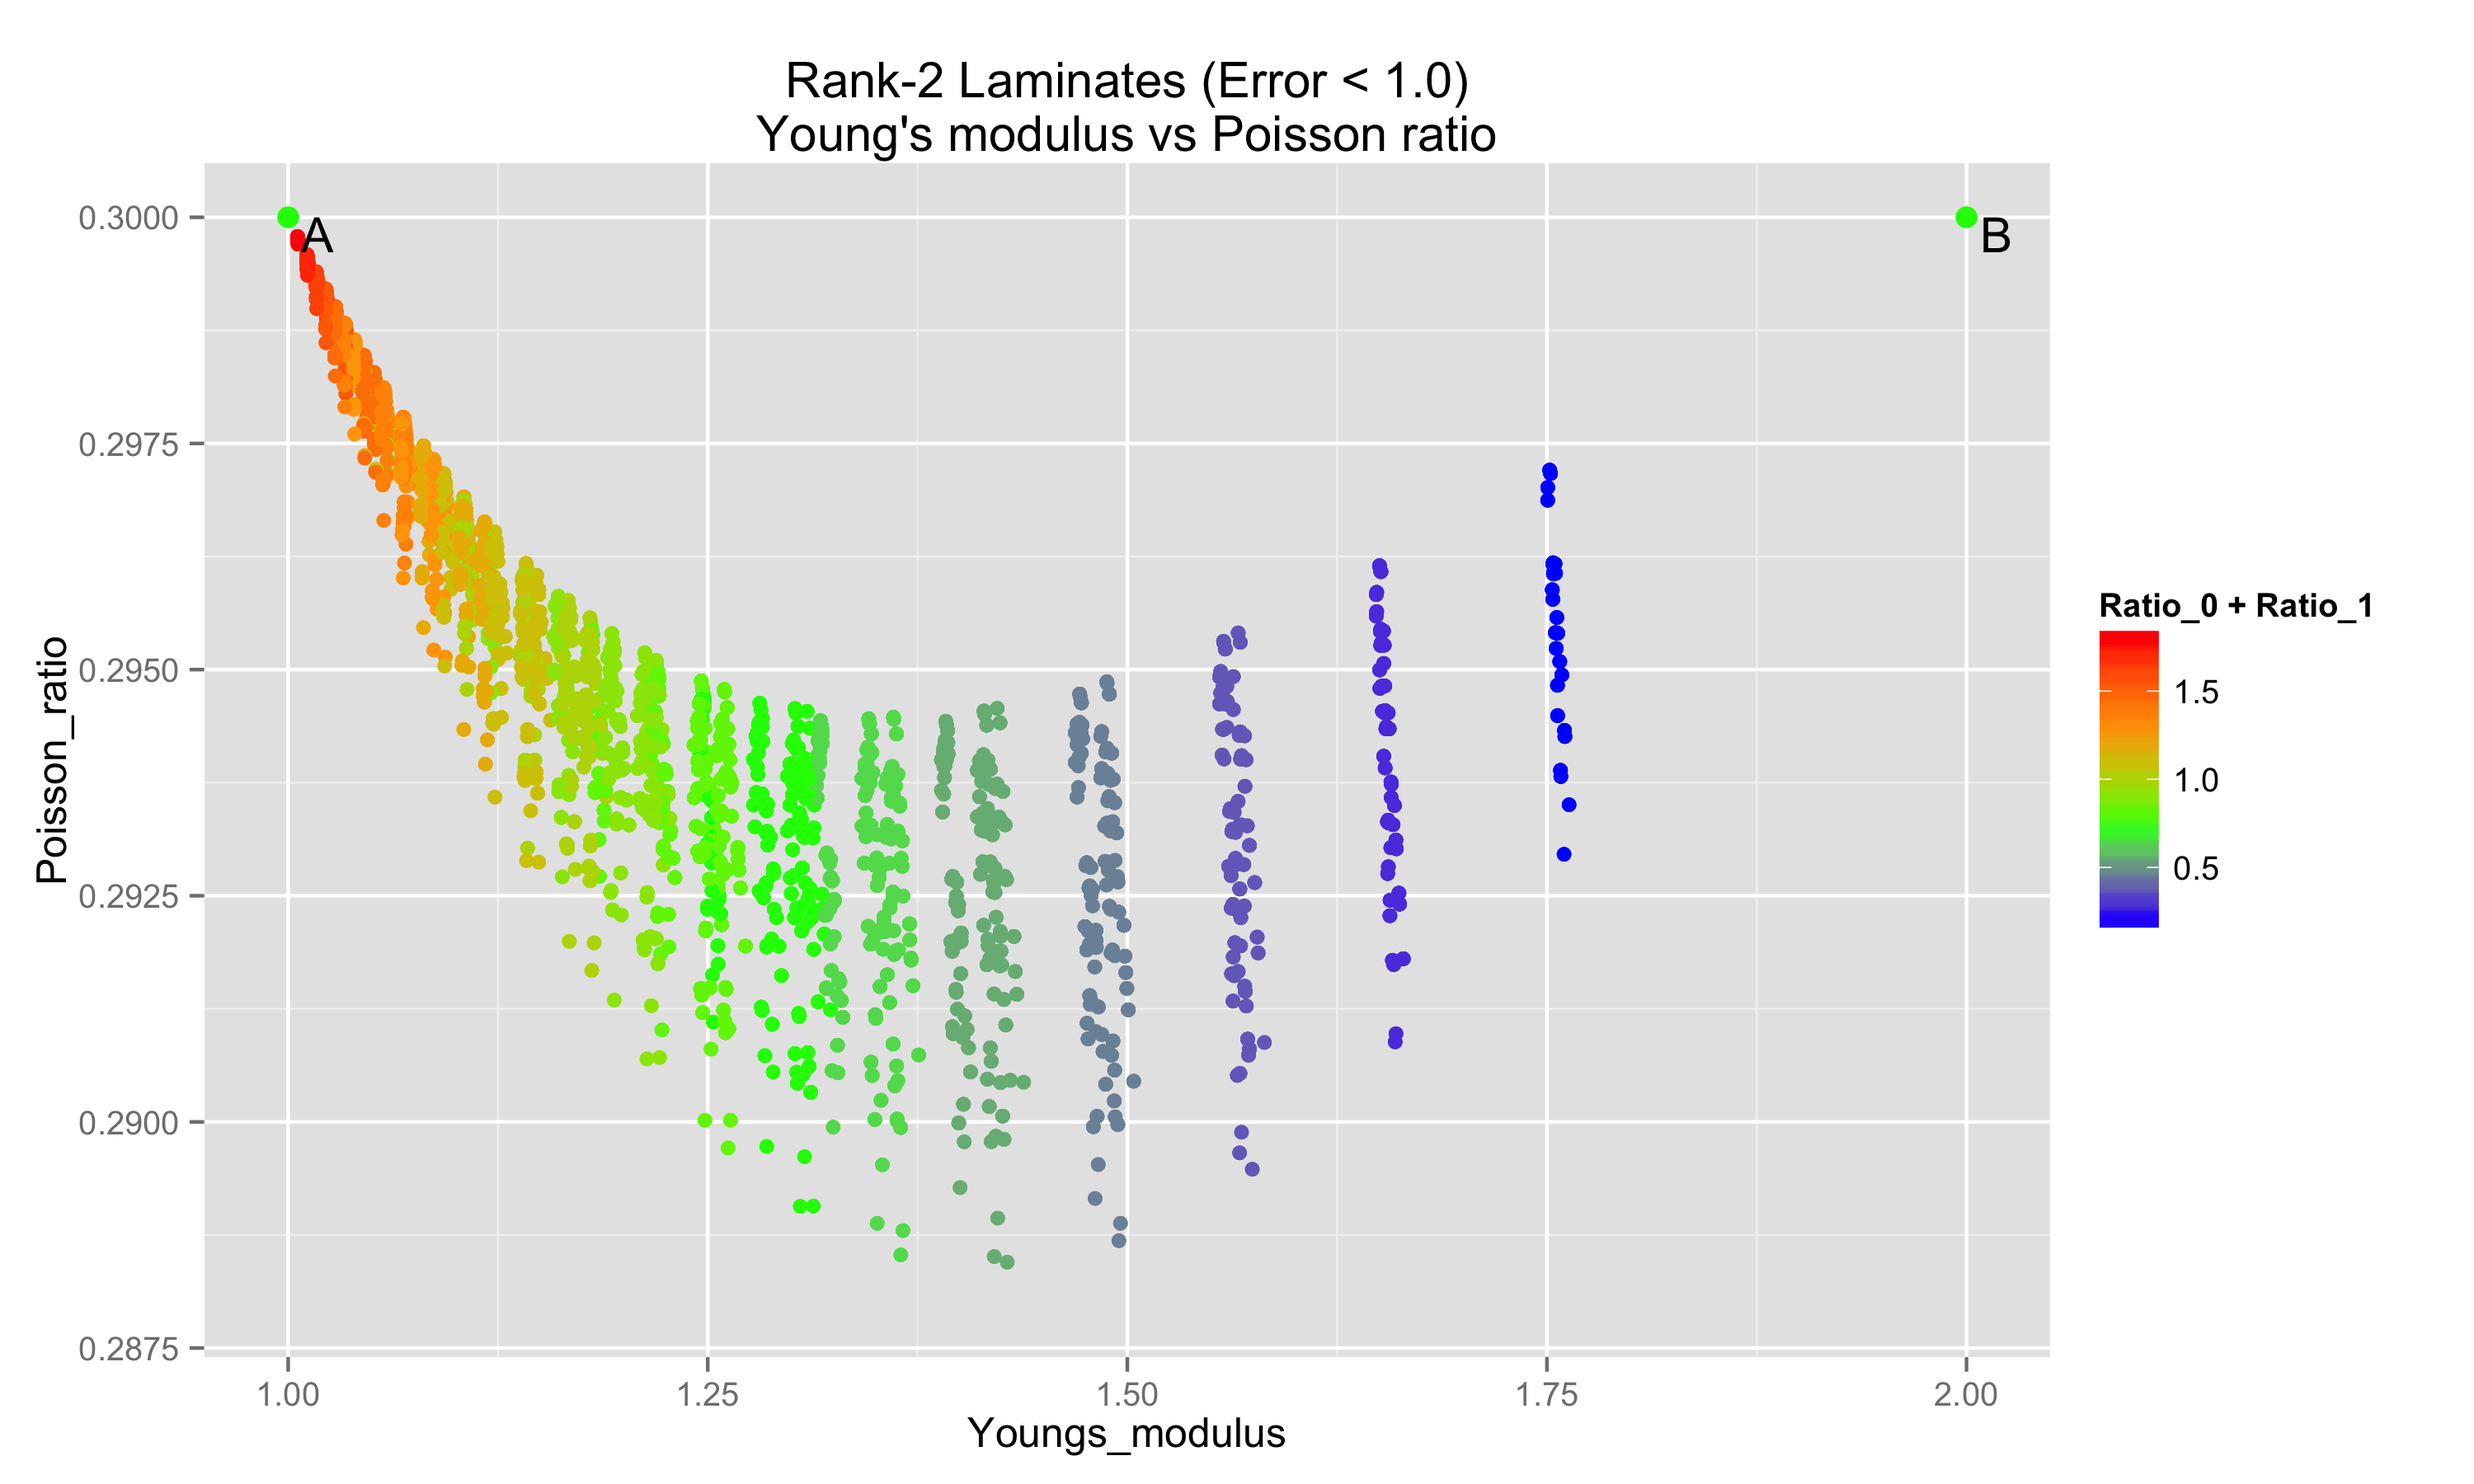
\includegraphics[width=0.49\textwidth]{{images/p2_e1.0_young_poisson_ratio}.png}
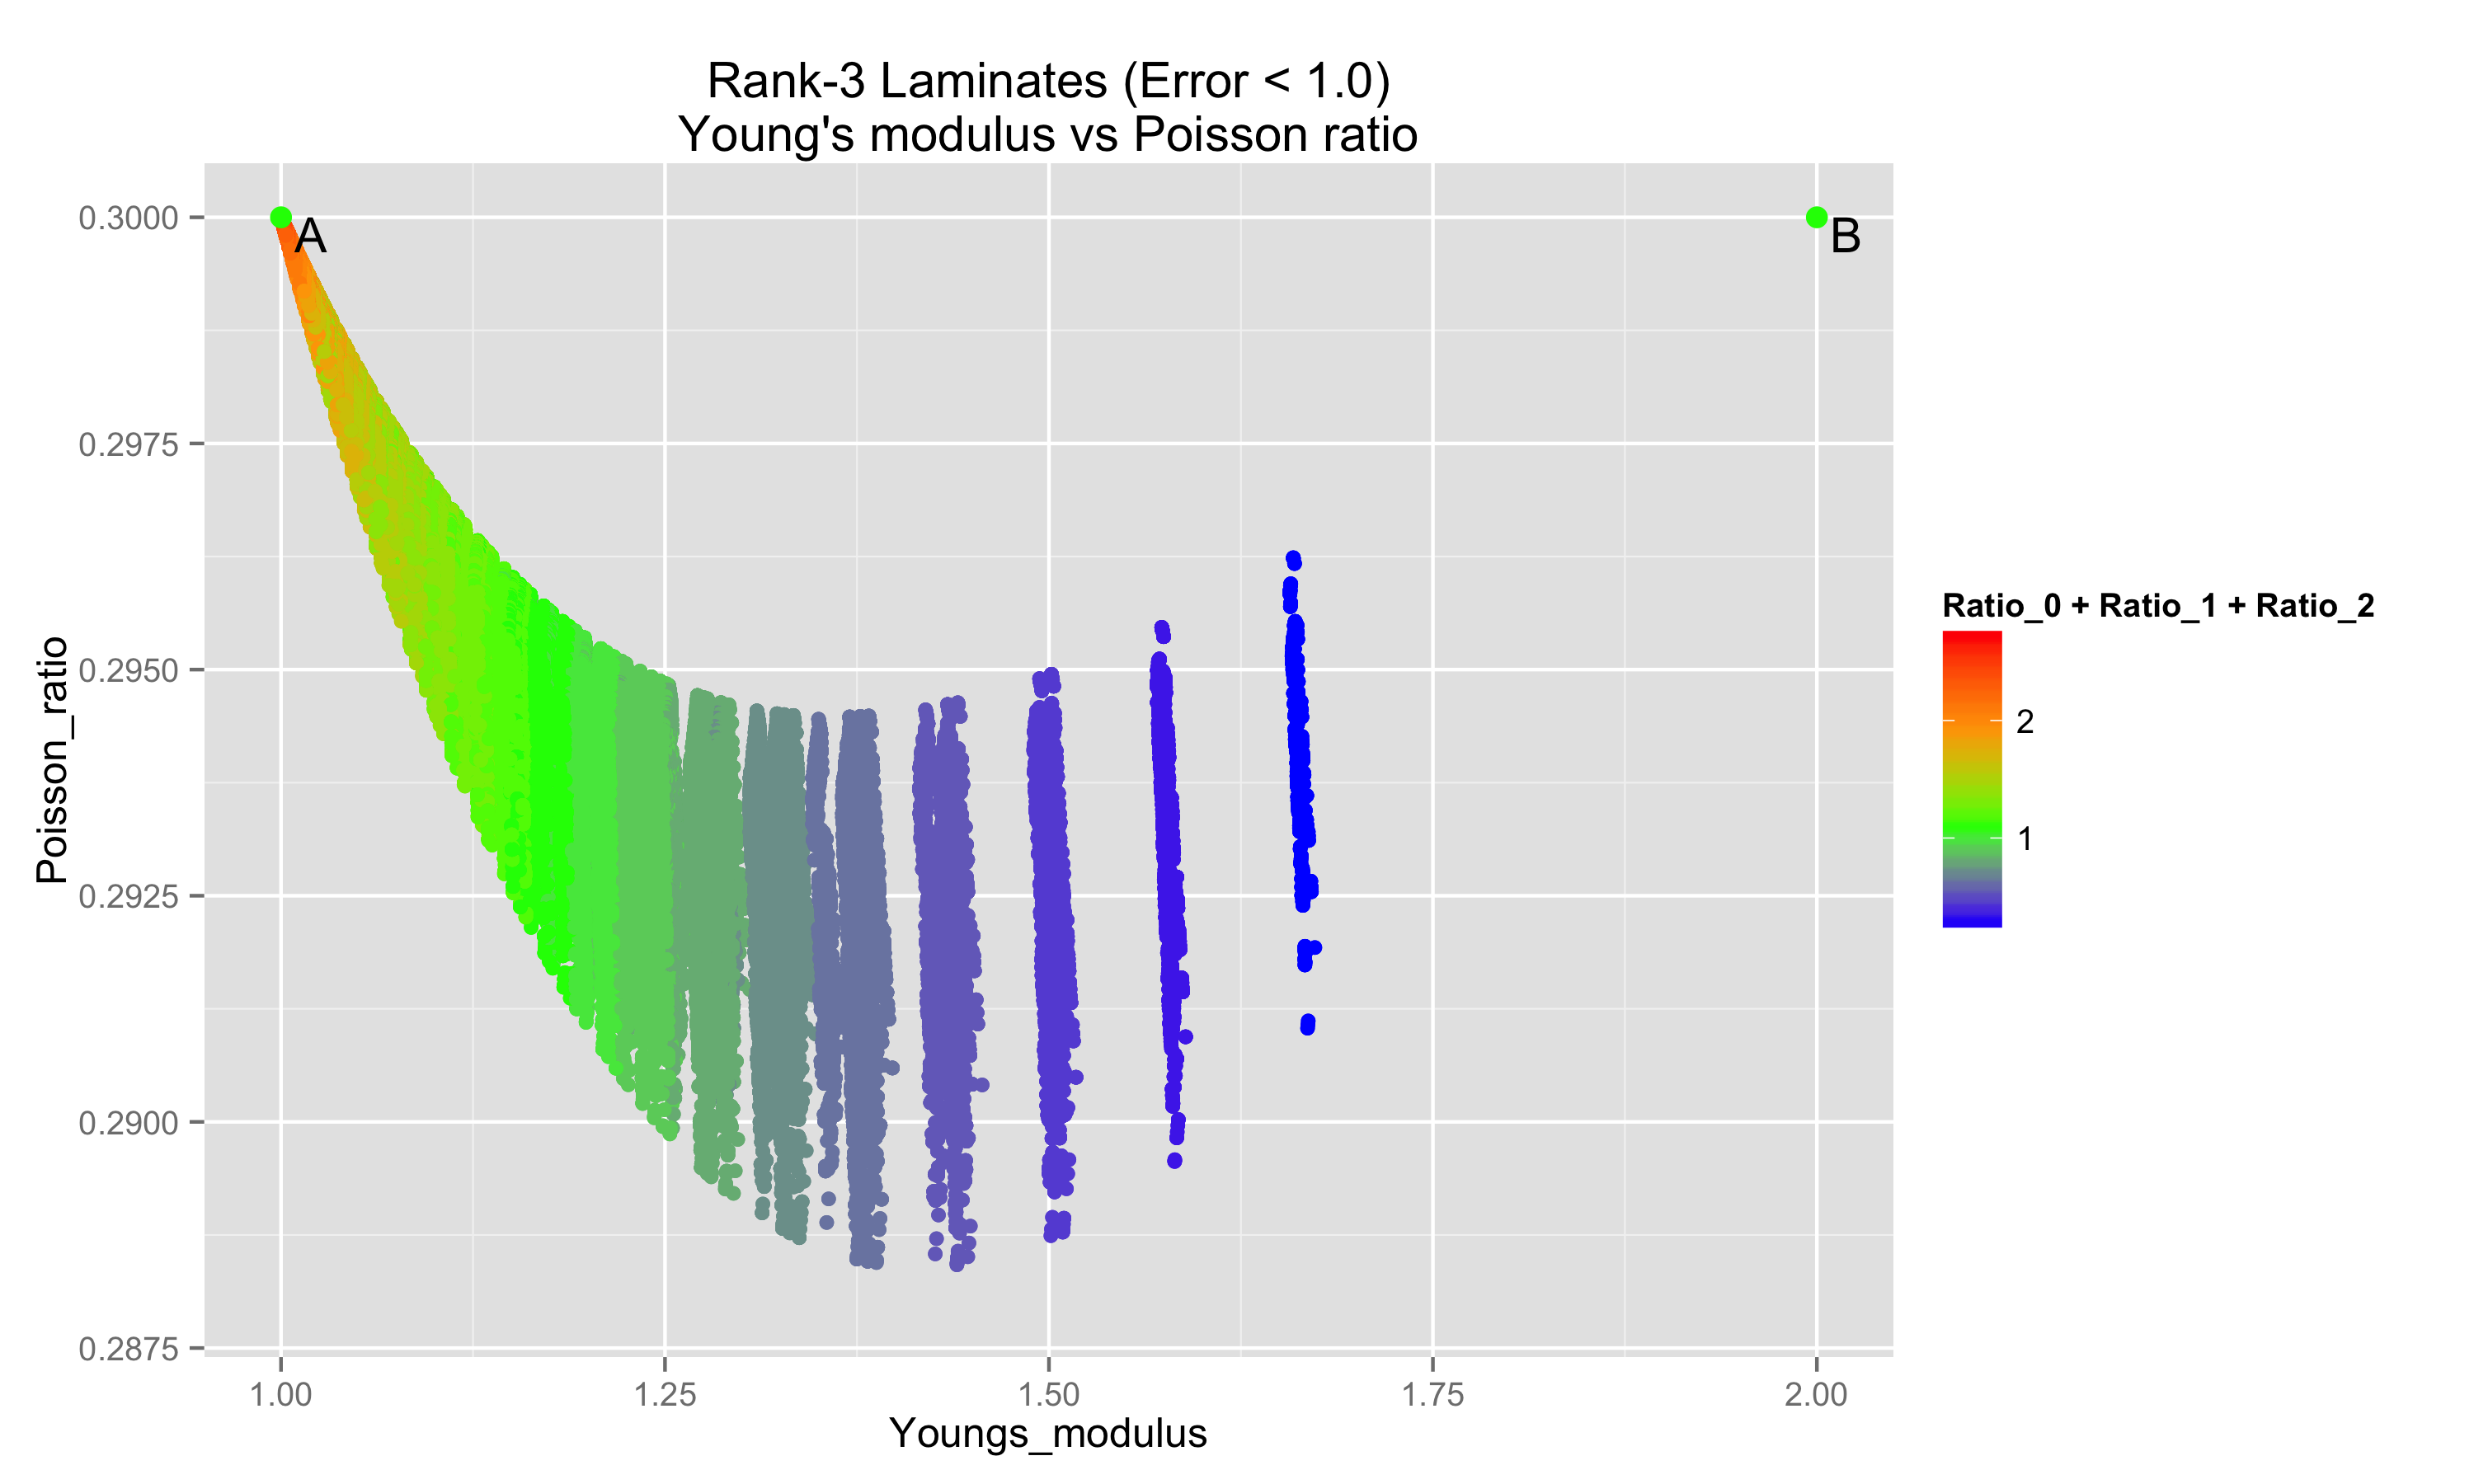
\includegraphics[width=0.49\textwidth]{{images/p3_e1.0_young_poisson_ratio}.png}
\caption{Homogenized material tensor of rank-2 (left) and rank-3 (right)
laminates visualized in Young's modulus vs Poisson ratio space.  Total material
ratio is ploted.  Notice that material ratio determines the Young's modulus of
the composite material.}
\label{fig:ratio}
\end{figure}

We also notice that the ratio of material dictates the Young's modulus of the
homogenized material.  Figure \ref{fig:ratio} shows all sampled material tensors
for rank-2 and rank-3 laminates with color representing the ratio of material
$A$.  All laminates with the same ratio of material A have roughly the same
Young's modulus.  Their Poisson ratios, howver, are different depending on their
lamination directions.

\begin{figure}
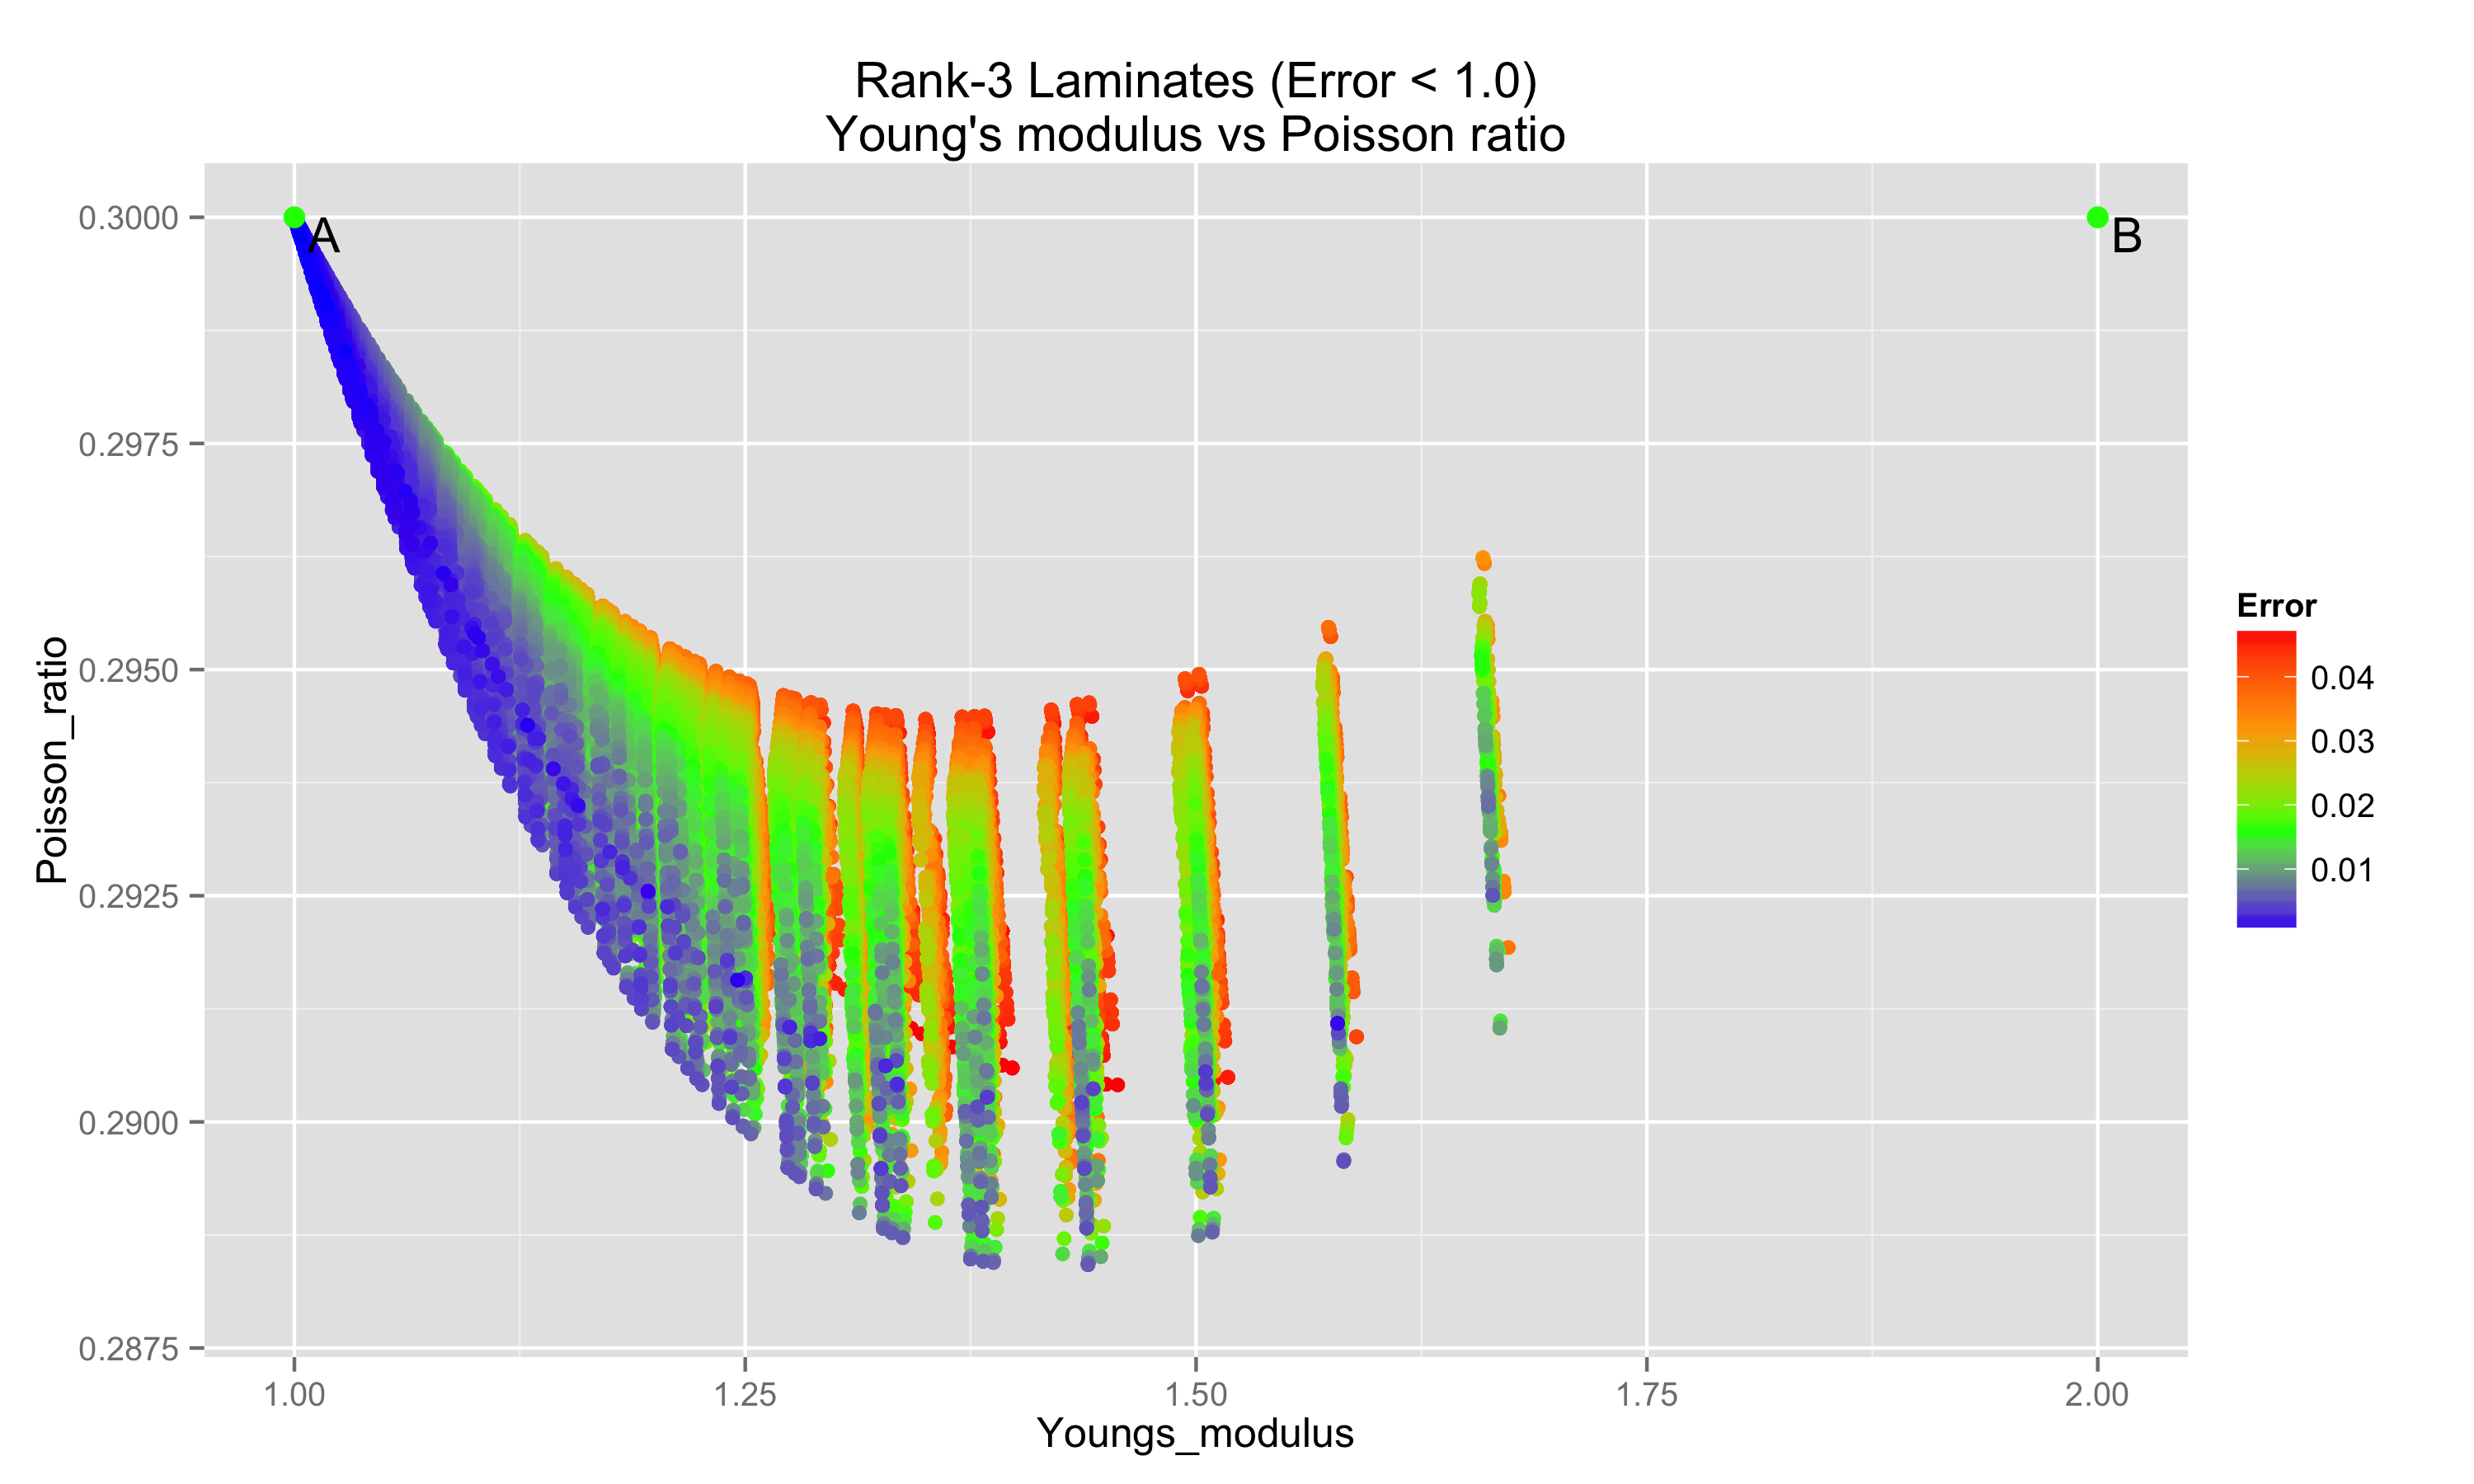
\includegraphics[width=0.49\textwidth]{{images/p3_e1.0_young_poisson_error}.png}
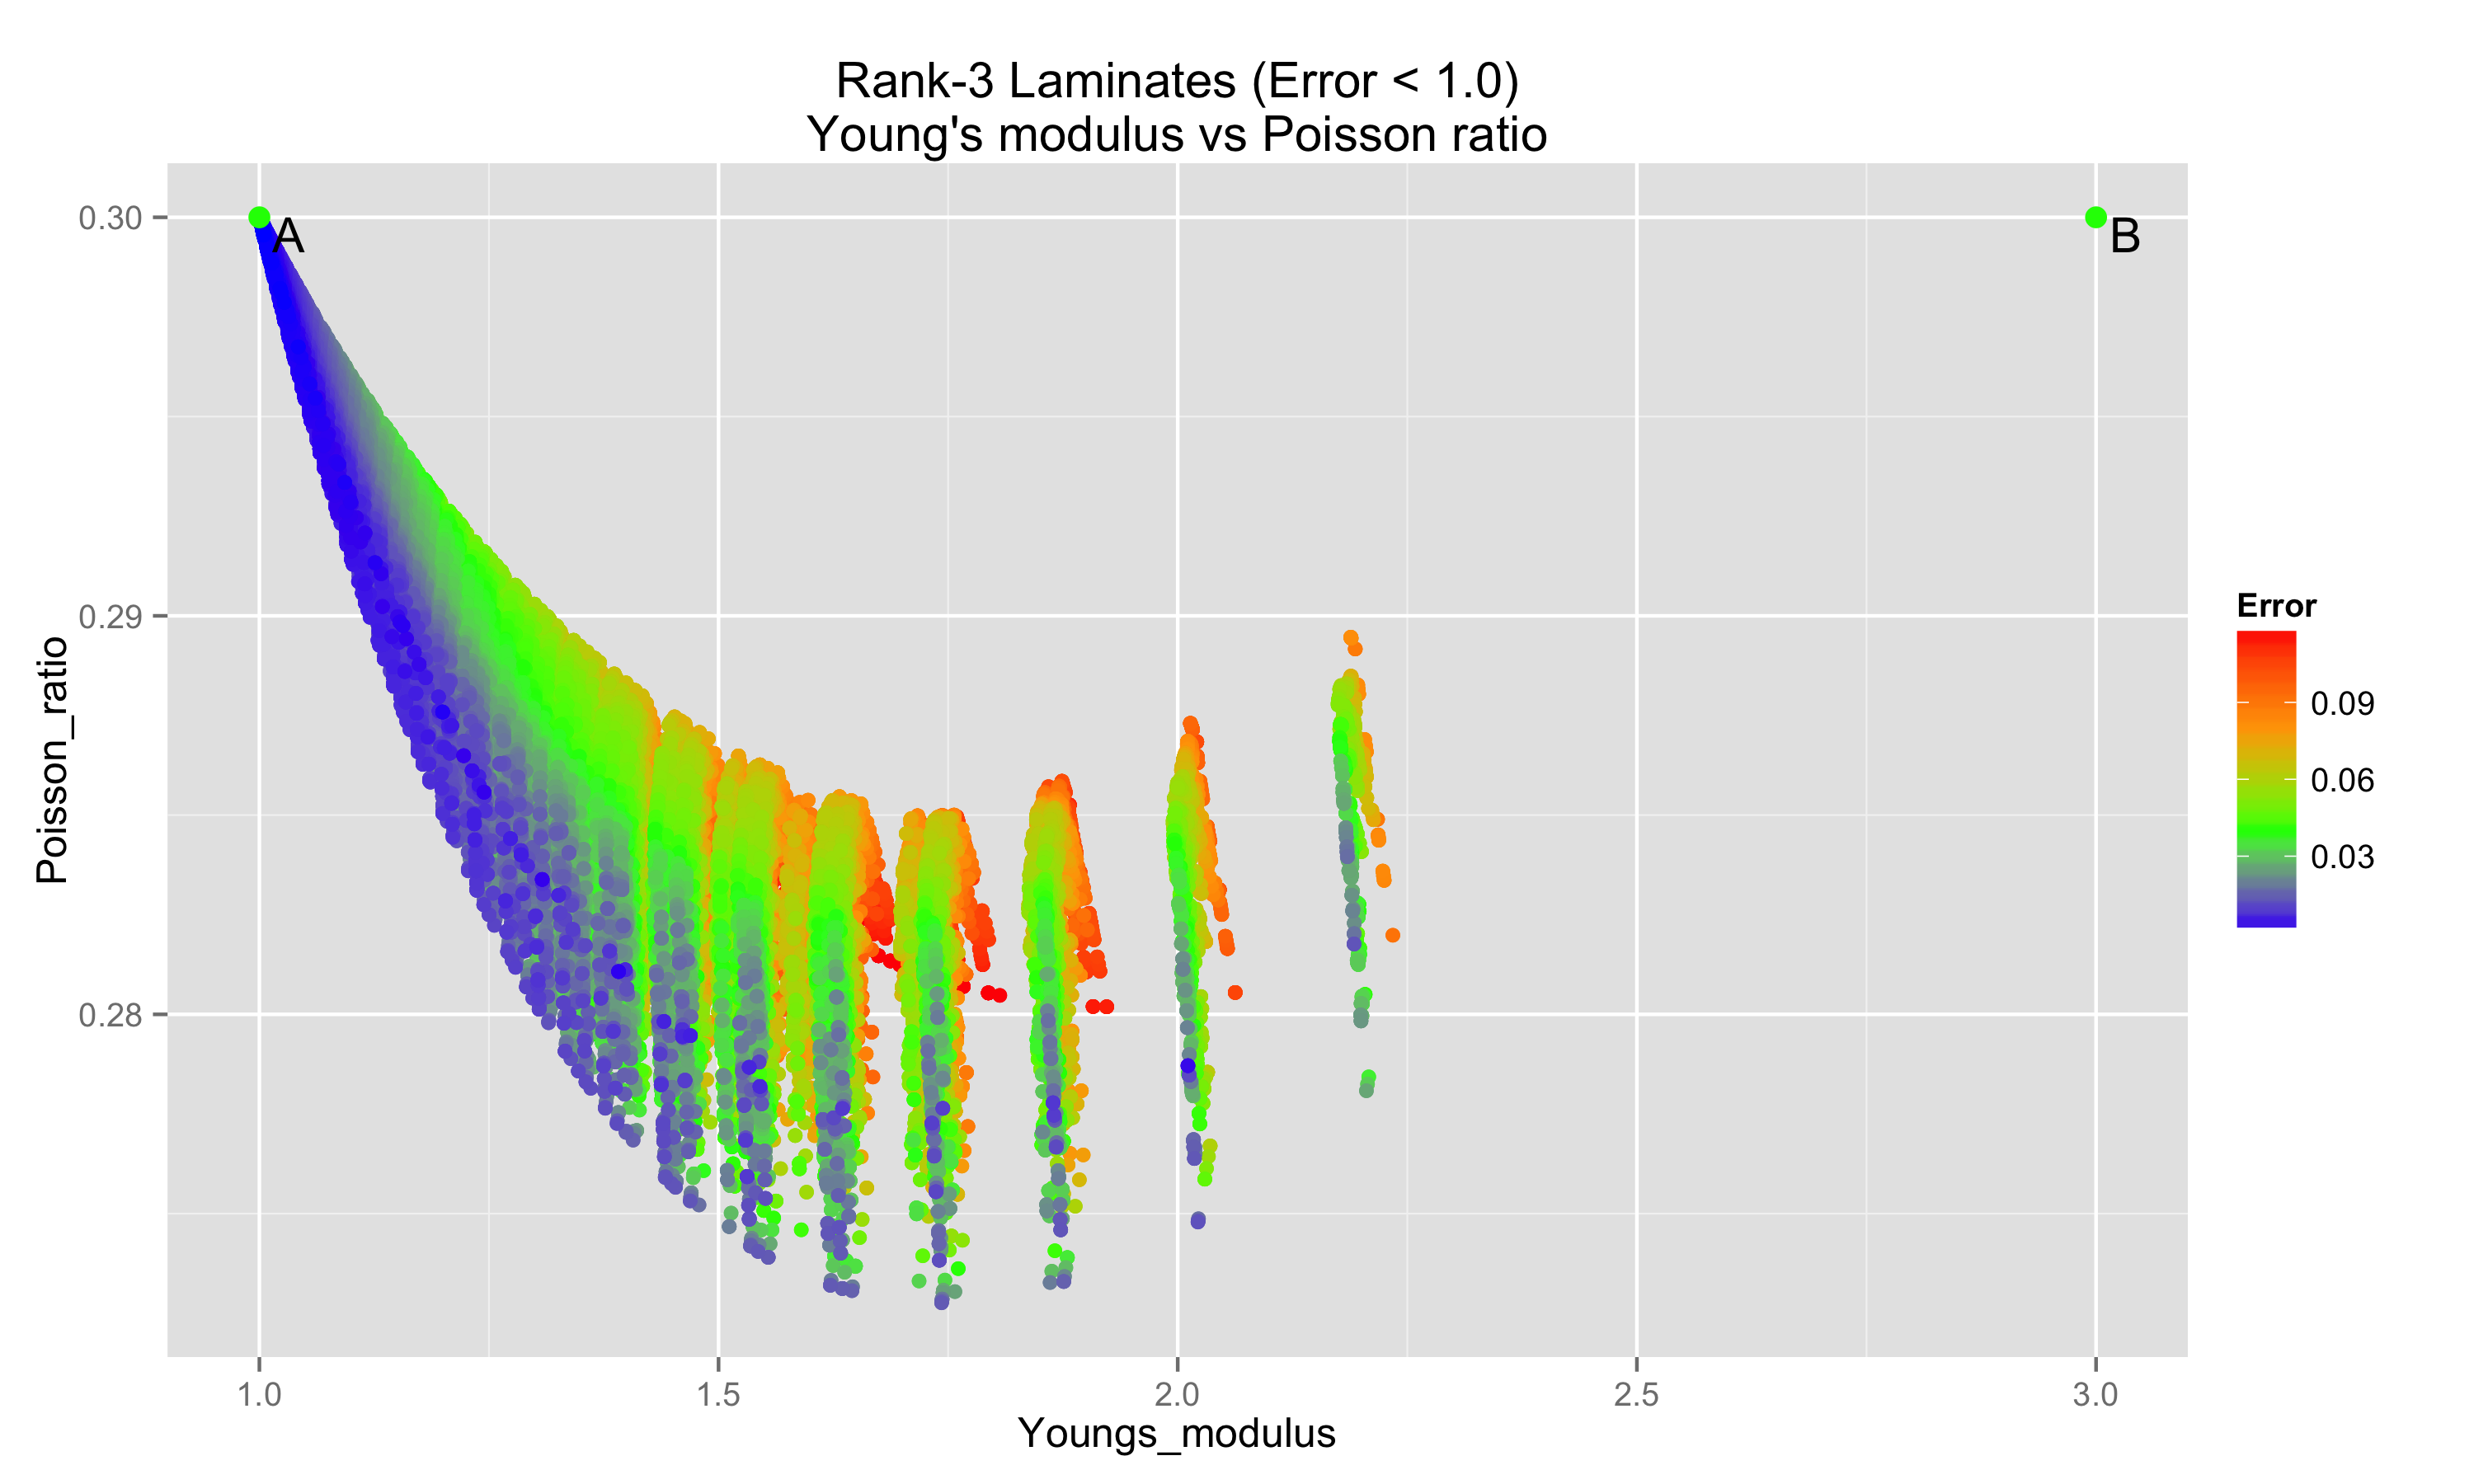
\includegraphics[width=0.49\textwidth]{{images/p3_e1.0_young_poisson_error_3.0}.png}
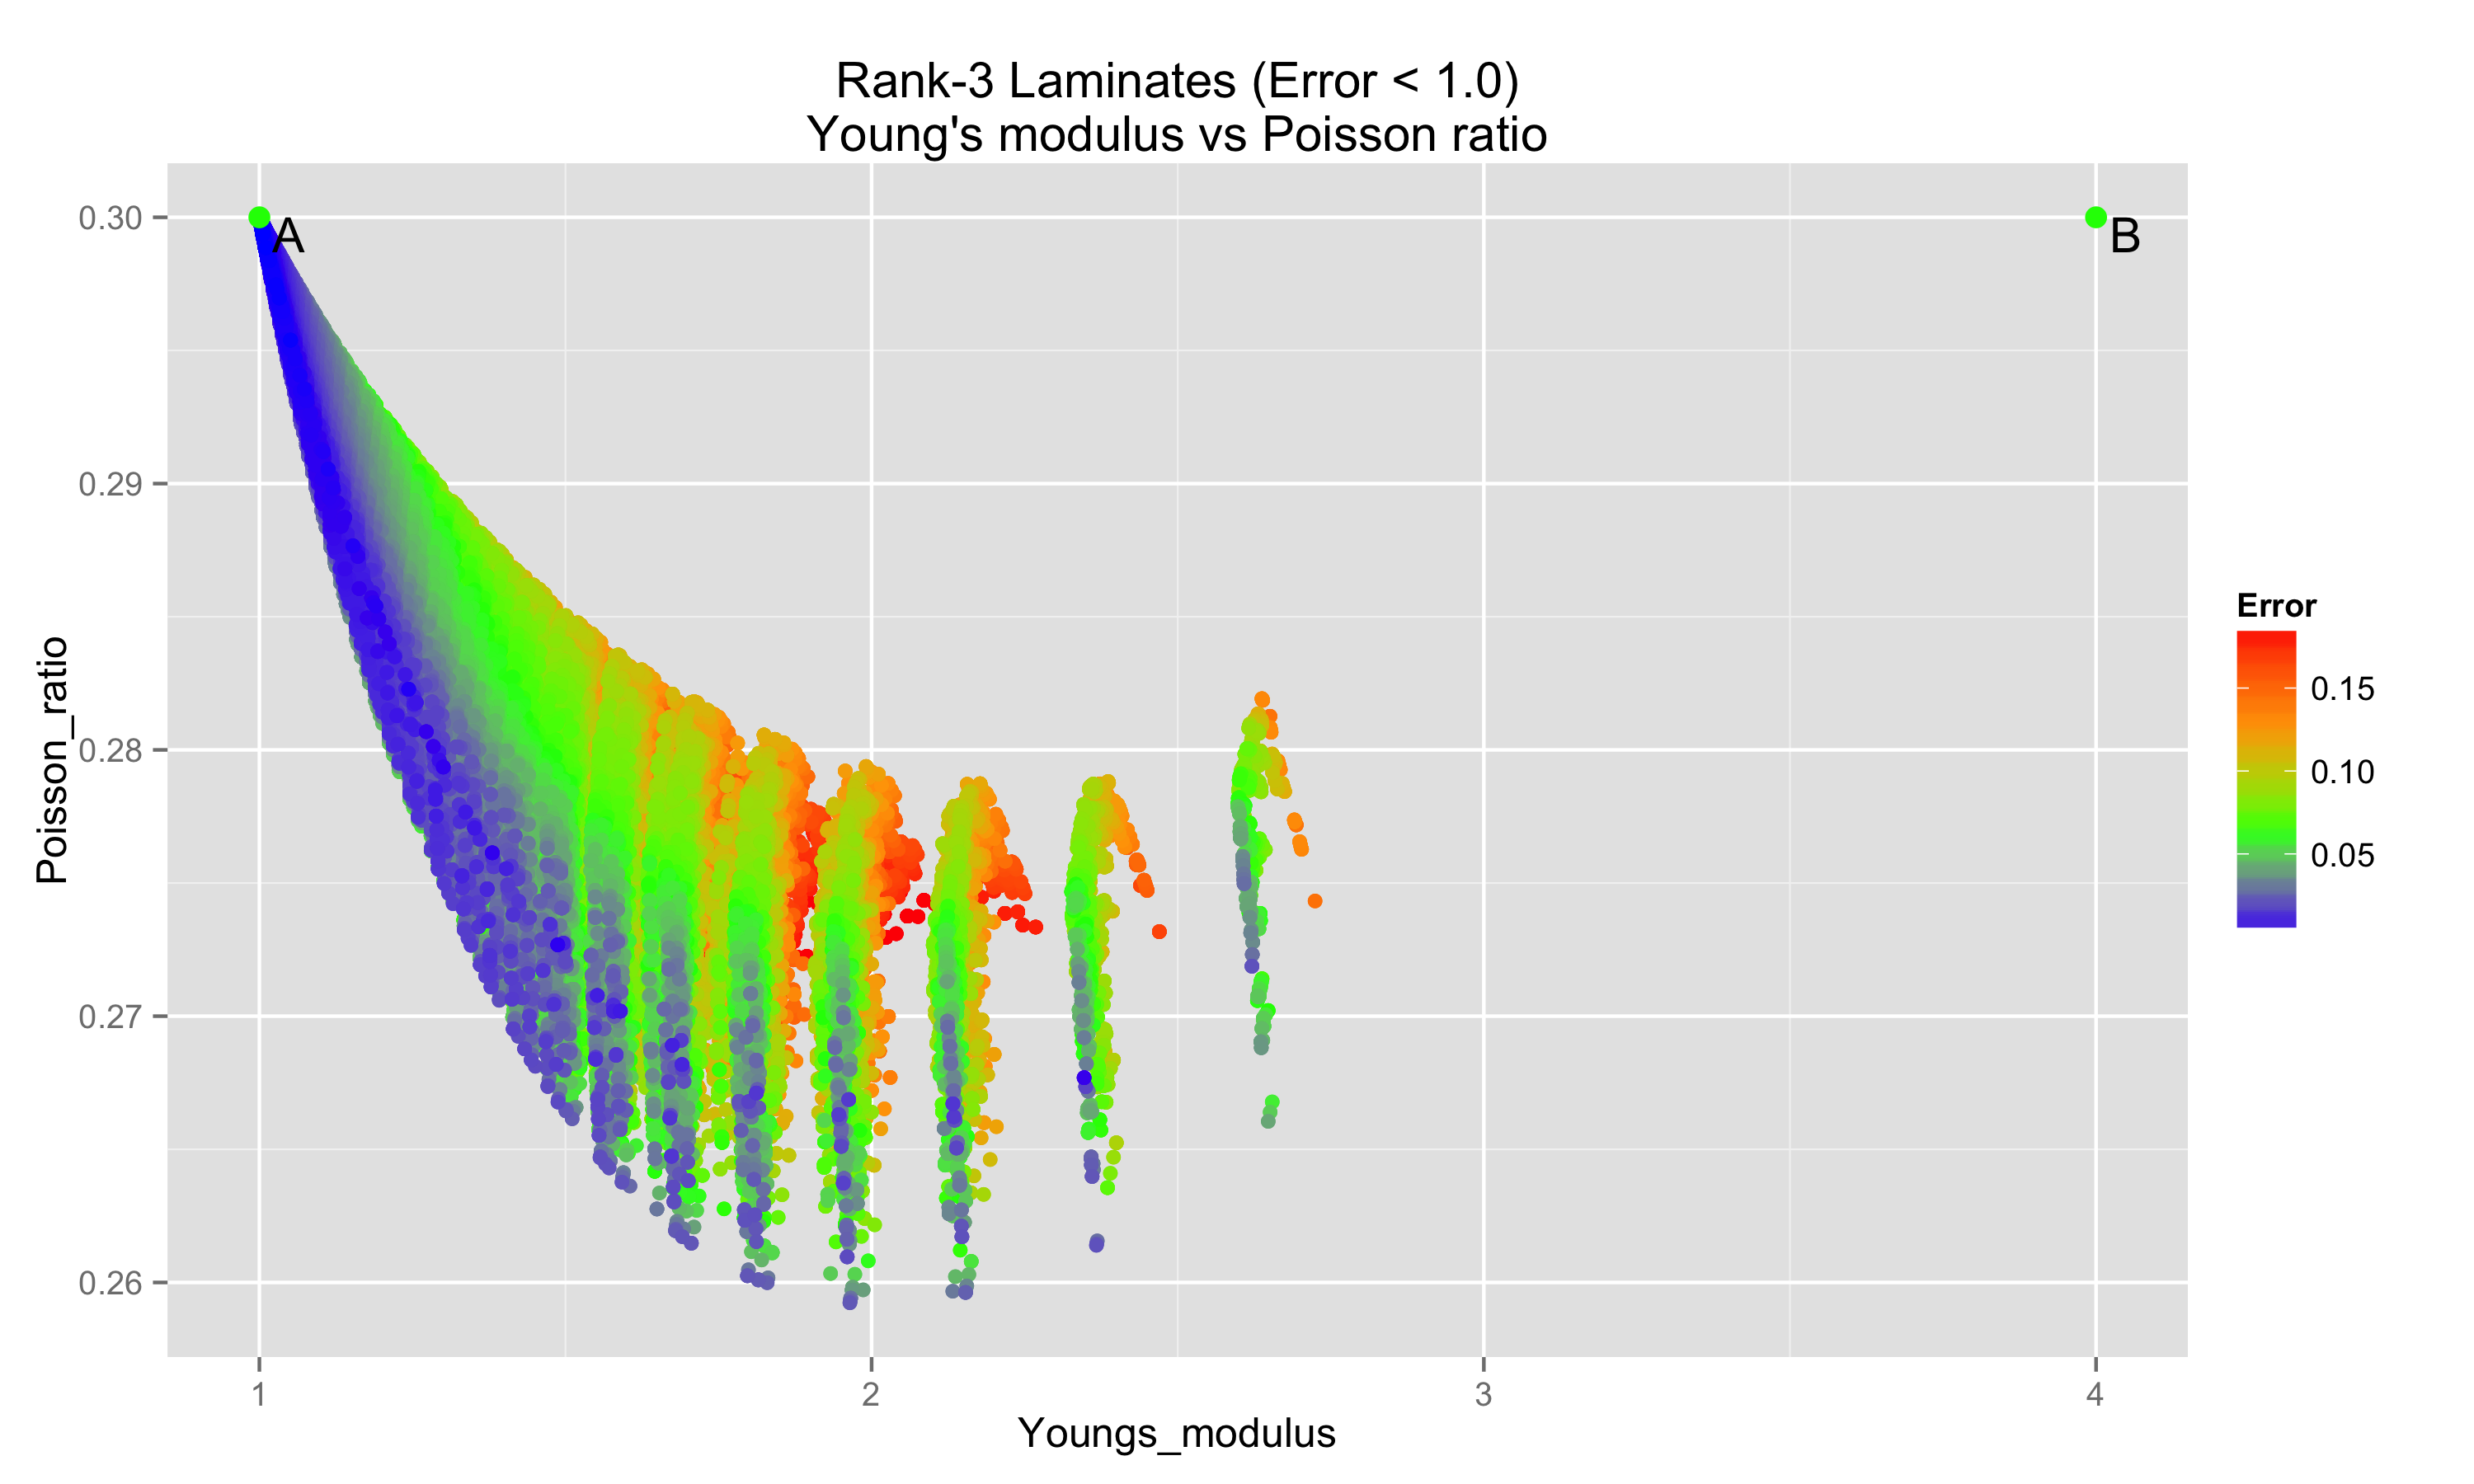
\includegraphics[width=0.49\textwidth]{{images/p3_e1.0_young_poisson_error_4.0}.png}
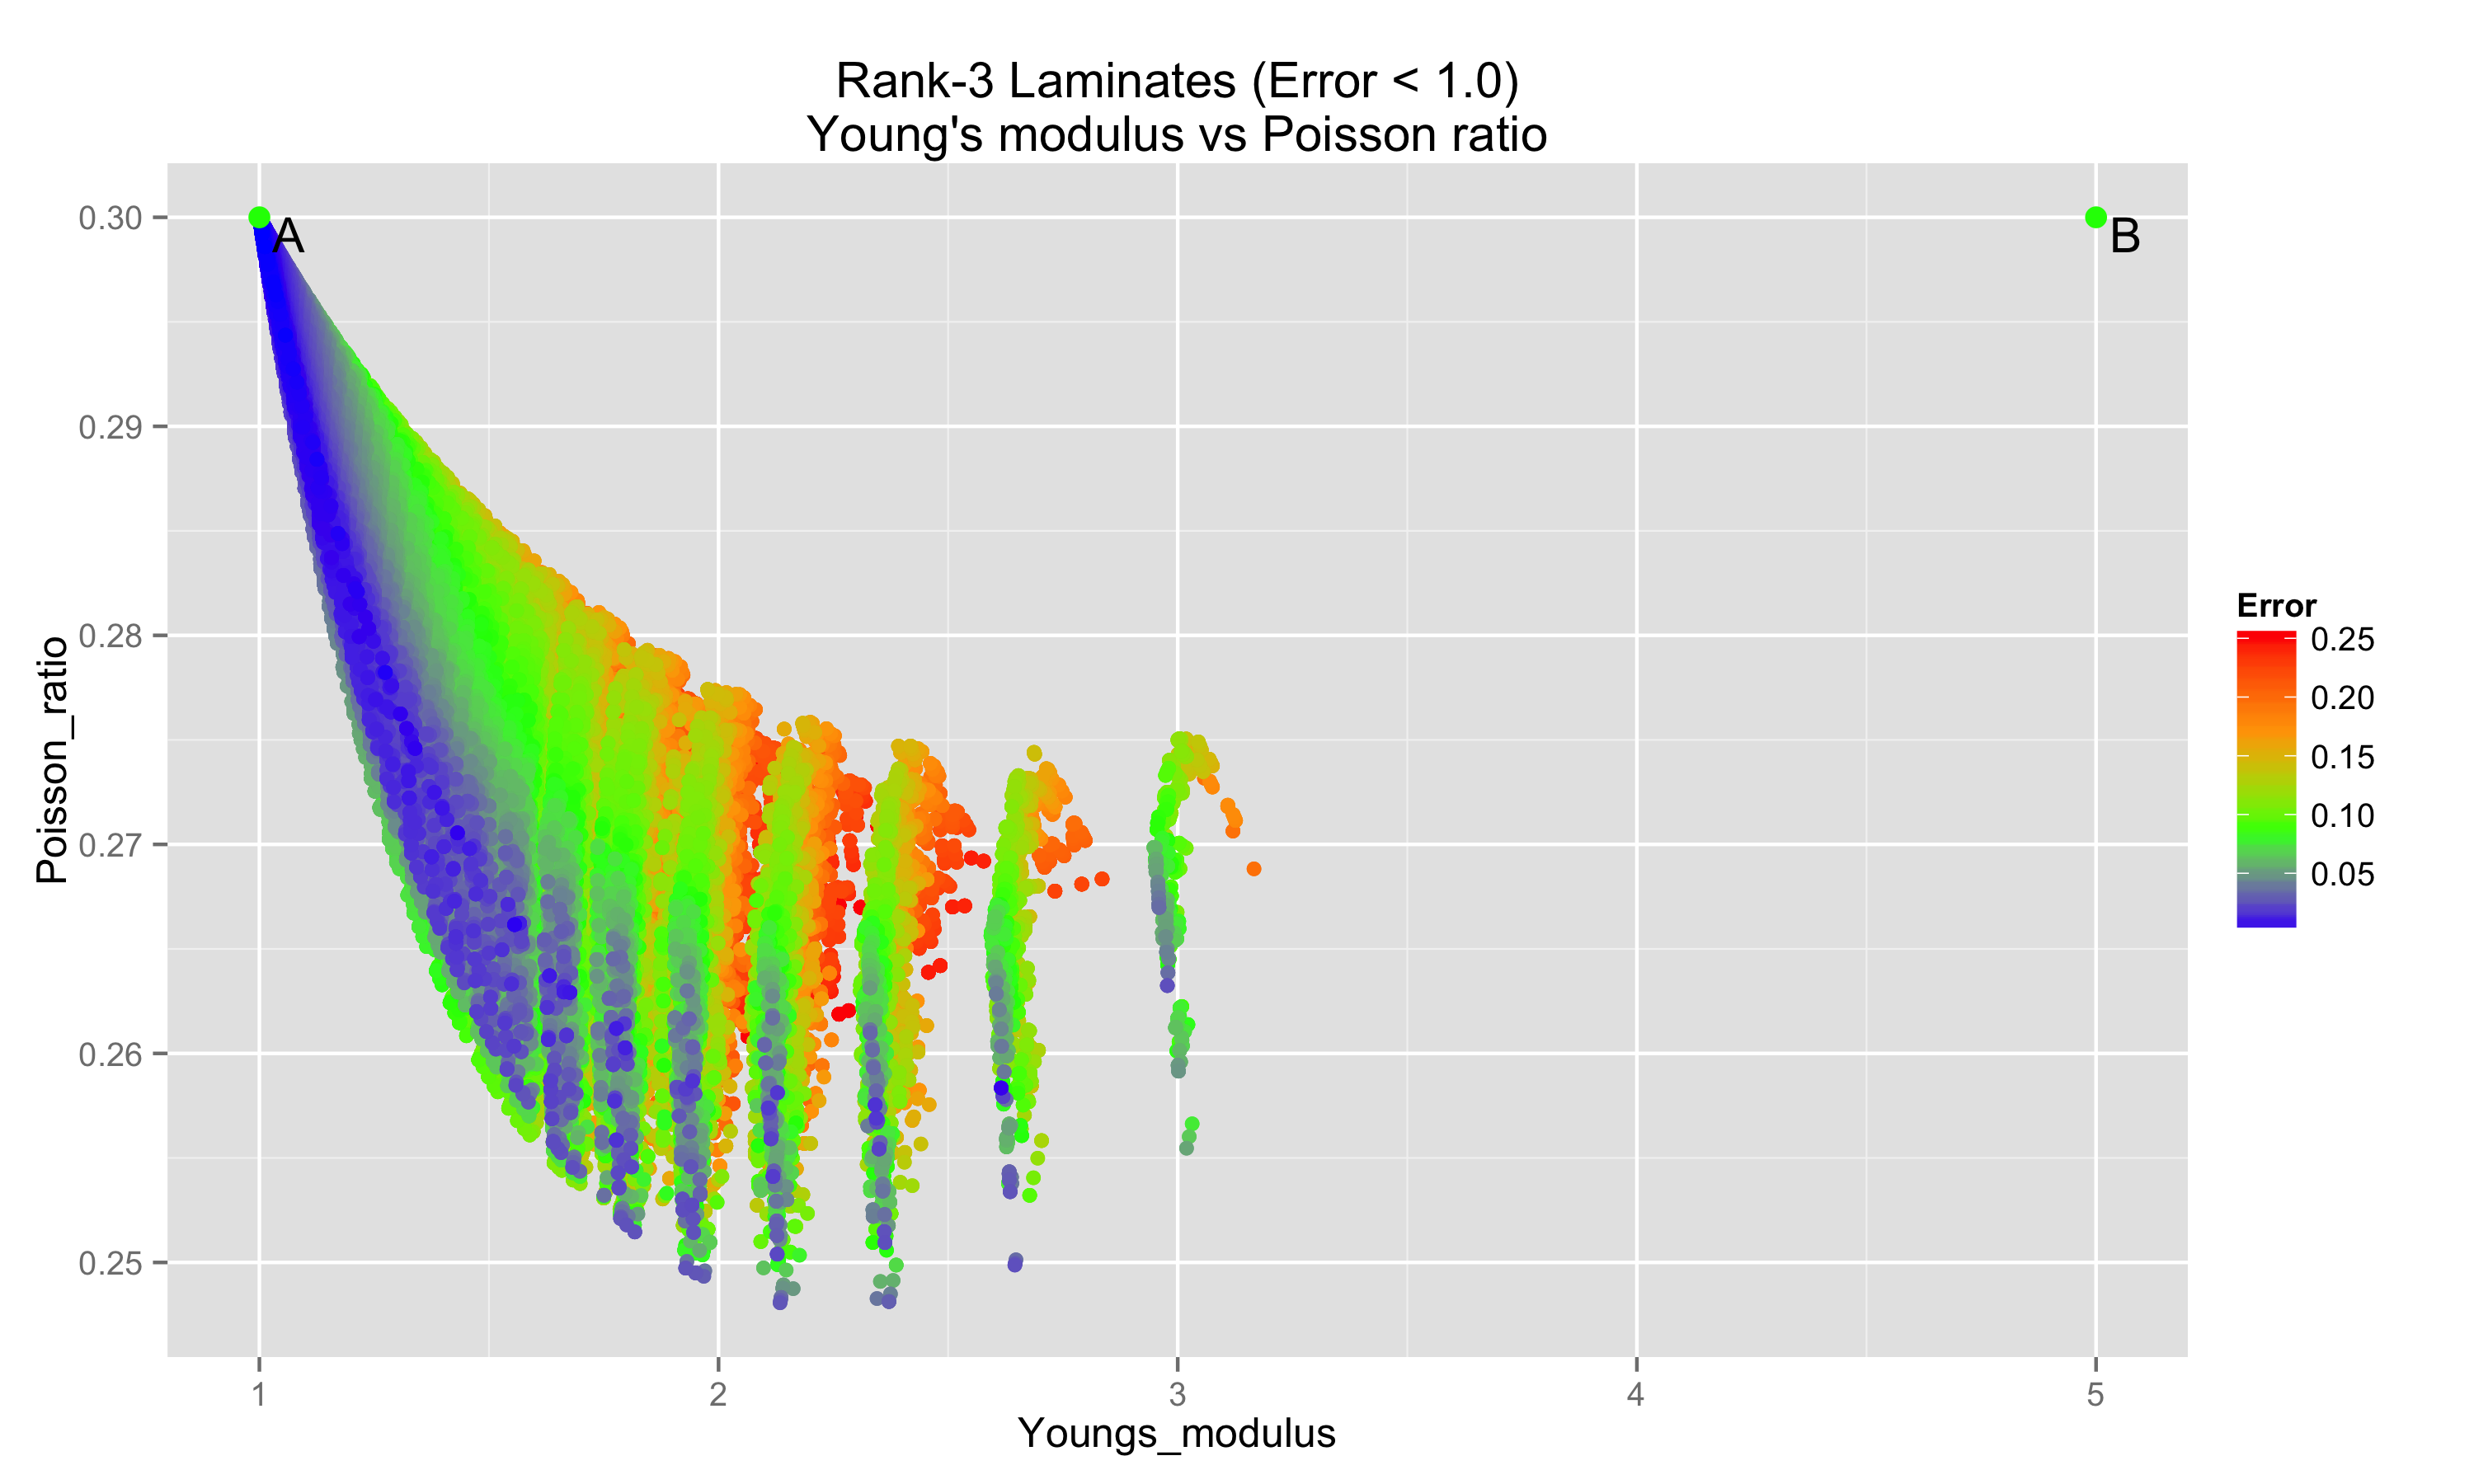
\includegraphics[width=0.49\textwidth]{{images/p3_e1.0_young_poisson_error_5.0}.png}
\caption{Homogenized material tensors of rank-3 laminates with different base
material $B$.  Color maps to fitting error. Top left: $E_B = 2$, Top right: $E_B
= 3$, Bottom left: $E_B = 4$, Bottom right: $E_B = 5$}
\label{fig:material_B}
\end{figure}

As we varies the base materials (Figure \ref{fig:material_B}), we observe that
the space occupies by homogenized material tensor remains crecent.  The more
isotropic samples points still concentrates near the lower arc of the crecent.

\begin{figure}
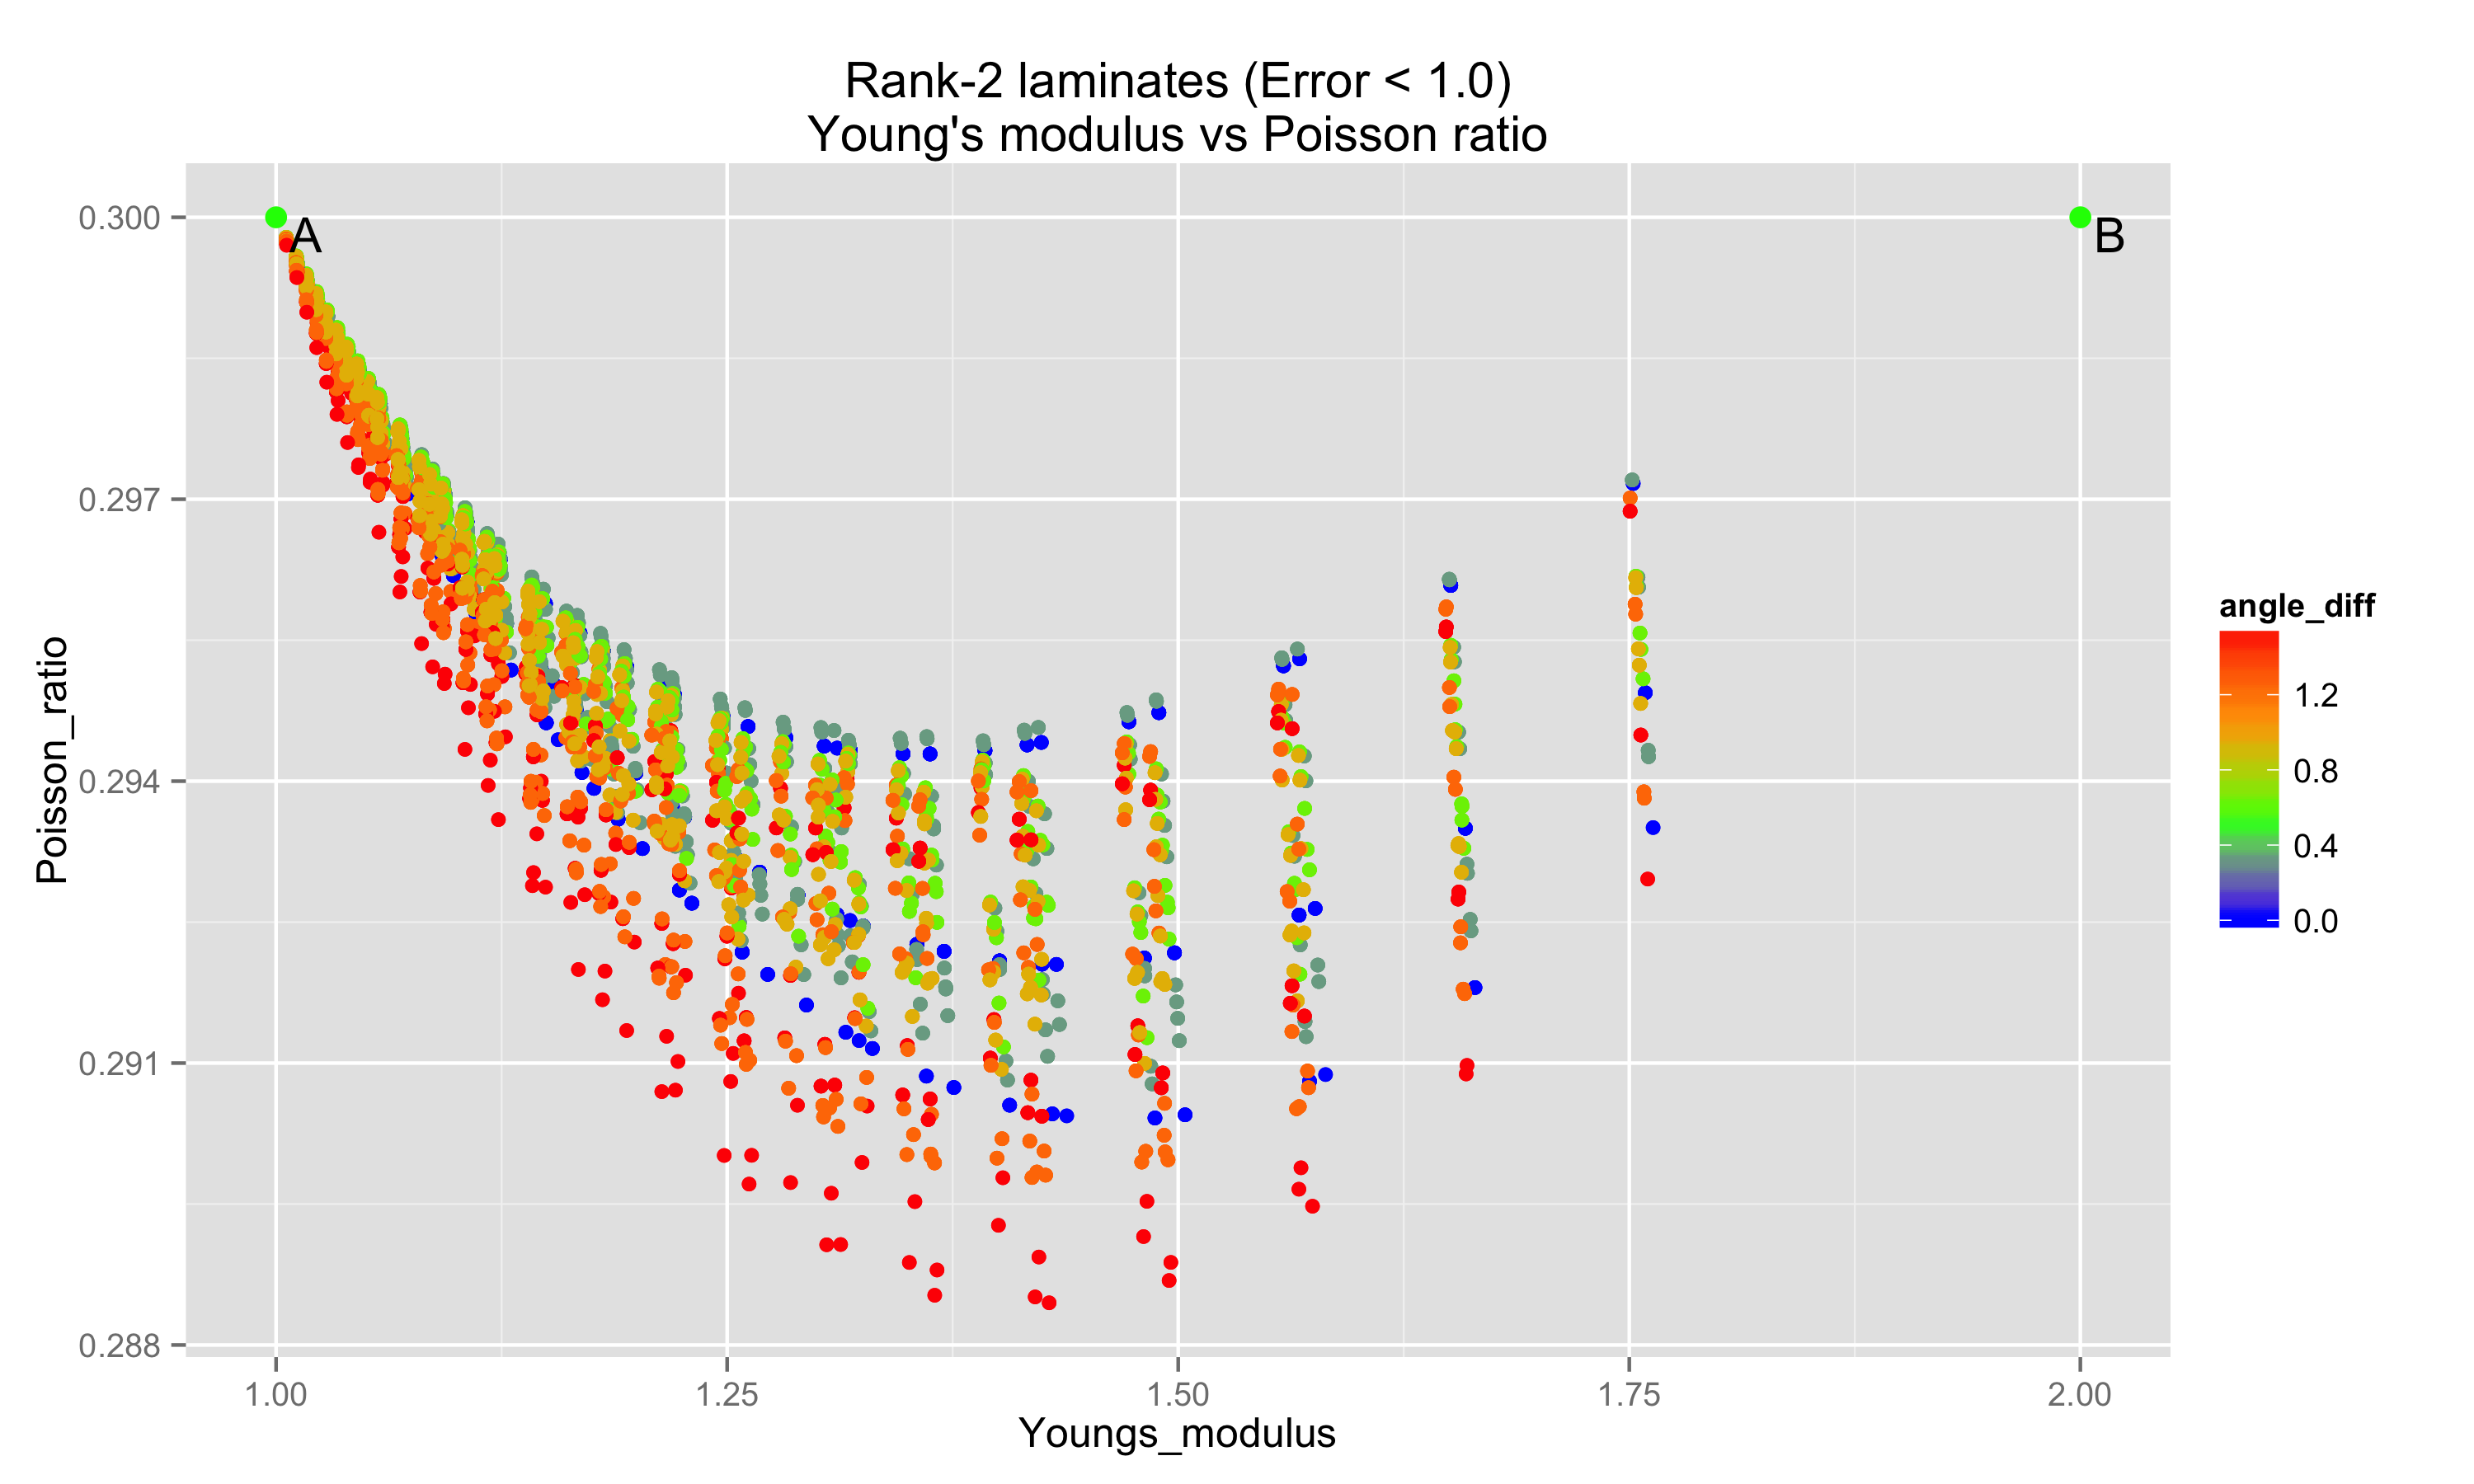
\includegraphics[width=0.49\textwidth]{{images/p2_e1.0_young_poisson_angle}.png}
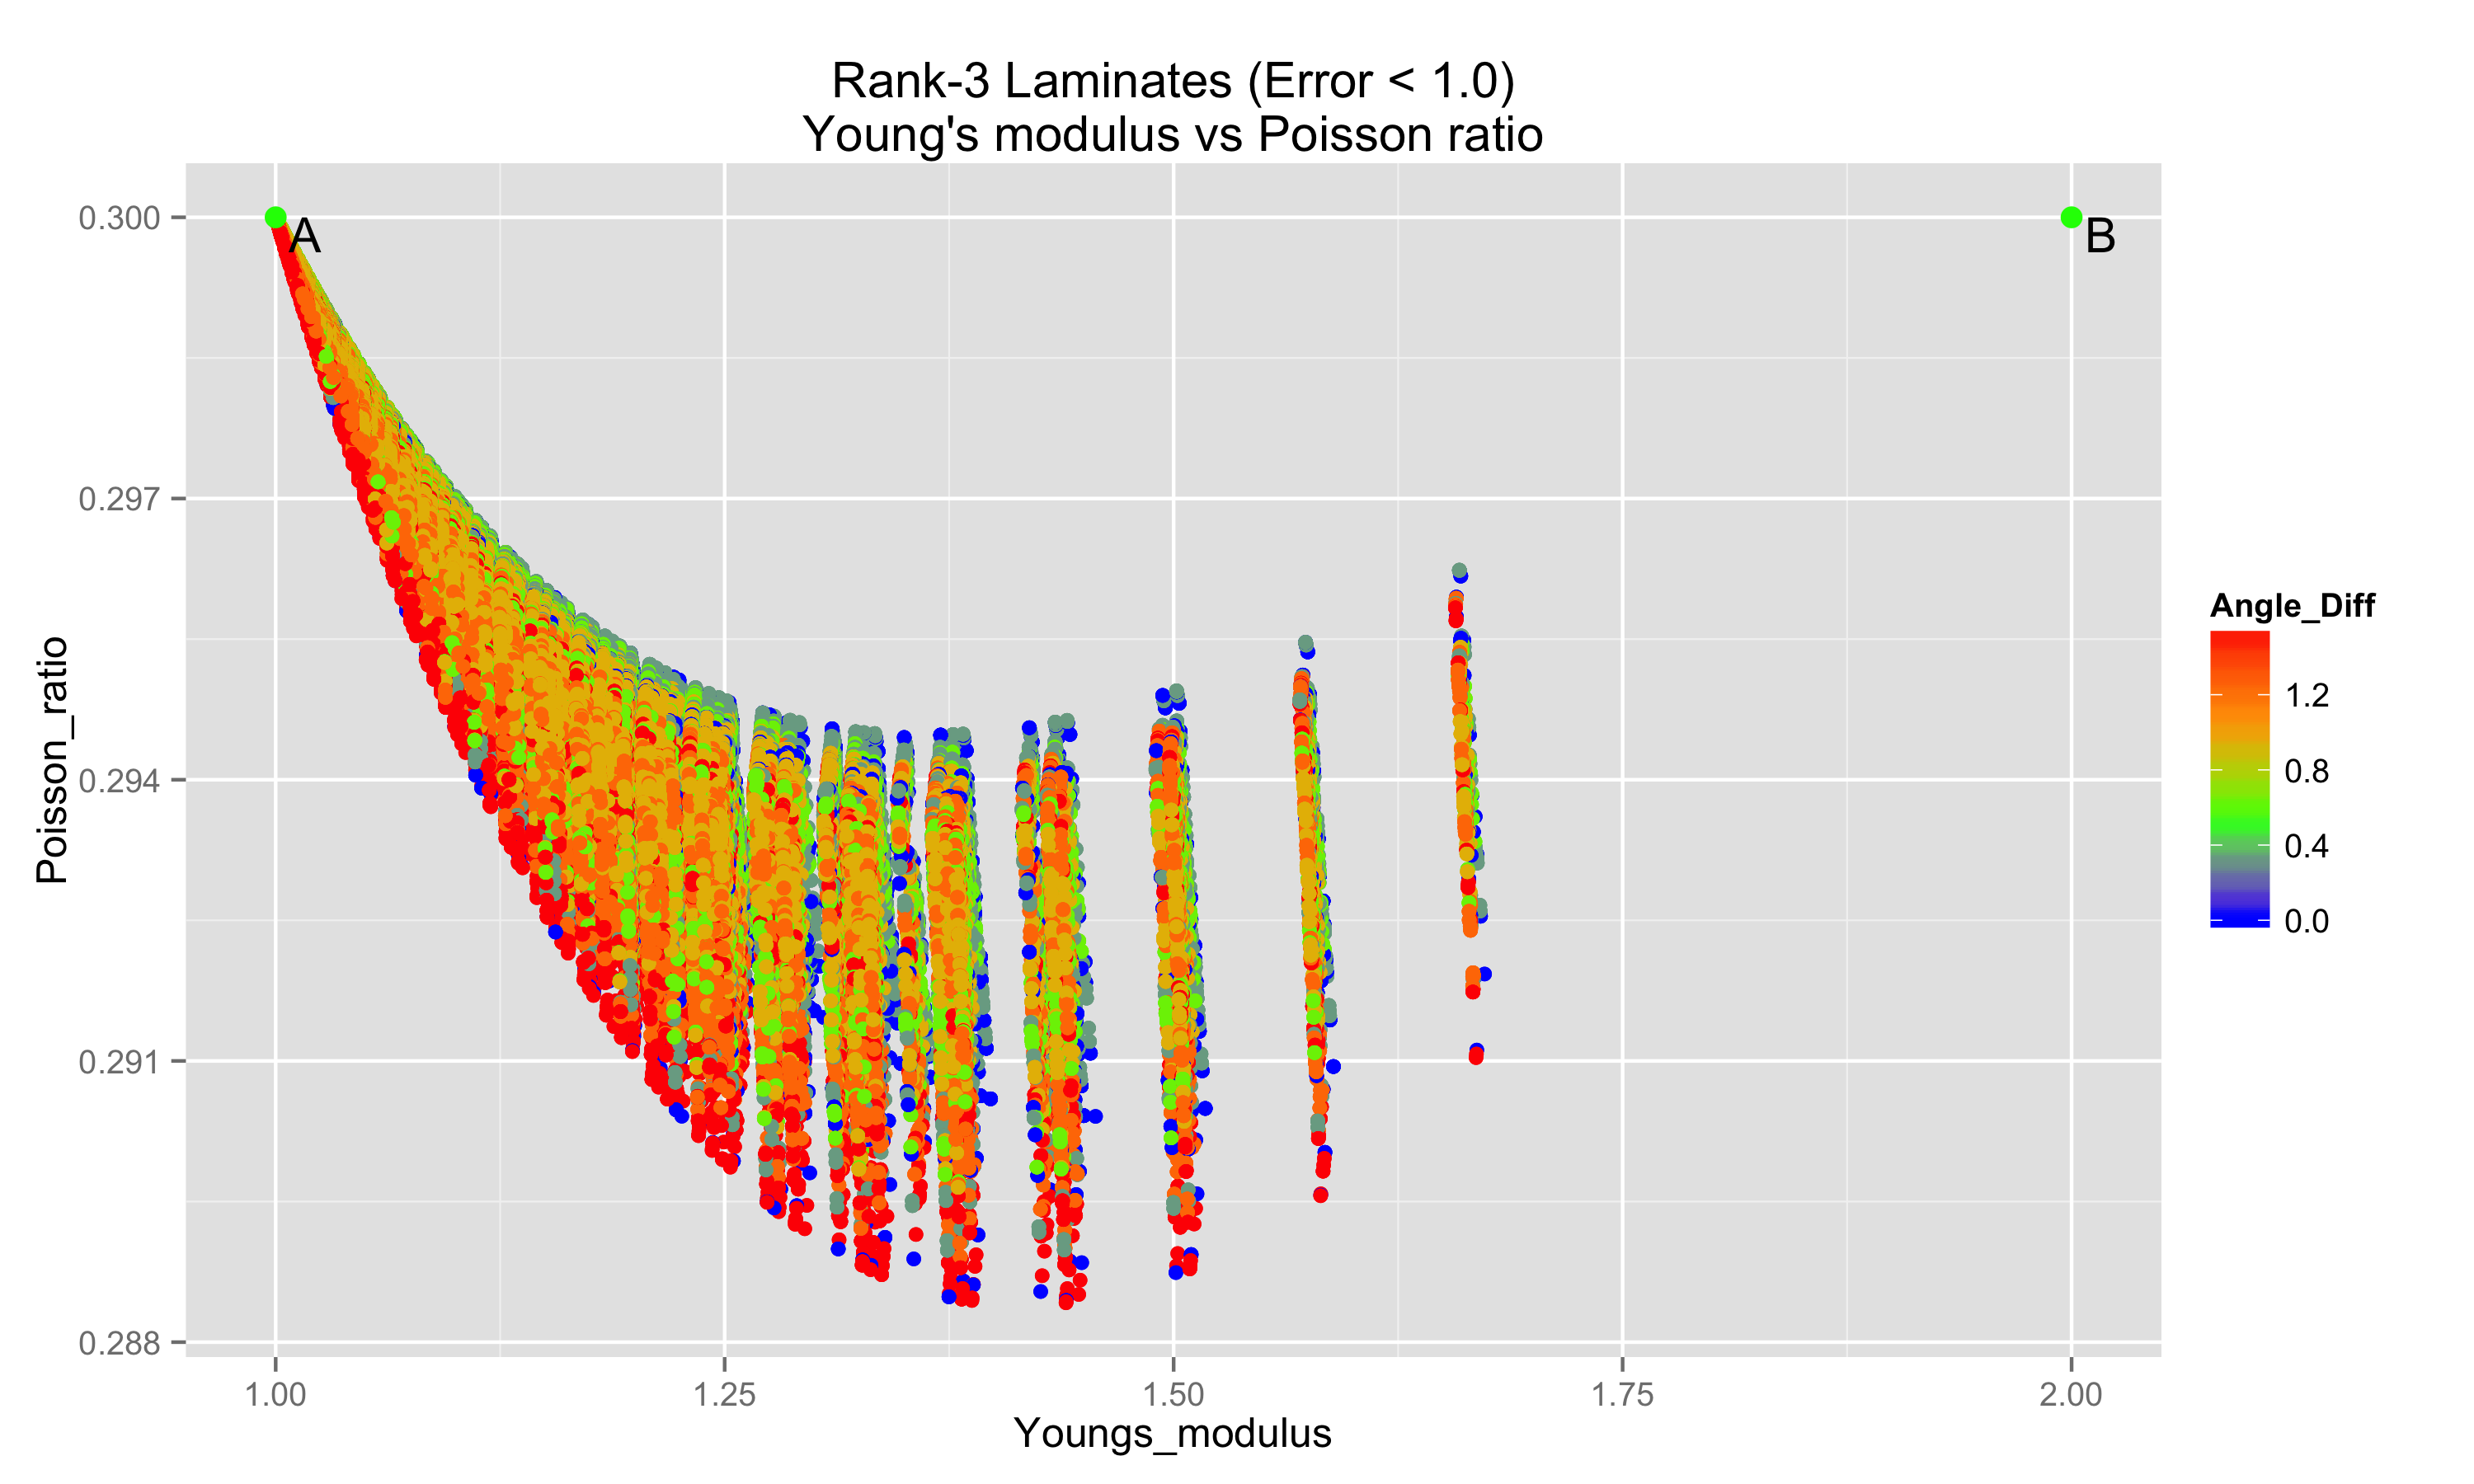
\includegraphics[width=0.49\textwidth]{{images/p3_e1.0_young_poisson_angle}.png}
\caption{The effect of relative lamination direction is shown here for rank-2
laminates (left) and rank-3 laminates (right).  For rank-3 laminates, we use the
relative lamination direction of the first 2 layers.}
\label{fig:angle_diff}
\end{figure}

For rank-2 laminates, we also explore the effect of the relative lamination
direction between the two layer on the resulting material.  Here relative
lamination direction is defined as $\alpha_{\textrm{diff}}$:
$$
\alpha_{\textrm{diff}} = \min(\abs{\alpha_0 - \alpha_1}, \pi - \abs{\alpha_0 -
\alpha_1})
$$
This quantity is visualized in Figure \ref{fig:angle_diff} (left).  Each
relative angle seems to determine an arc in the crecent space.  We also
attempted to visualize relative lamination direction of the first 2 layers for
rank-3 laminates (Figure \ref{fig:angle_diff} right), but result does not reveal
much.

\bibliographystyle{plain}
\bibliography{References}

\end{document}
